% General Configs

\documentclass[10pt, compress]{beamer}

%---------------------------------------------------------
%---------------------------------------------------------
\usepackage[alf]{abntex2cite}
\usepackage[utf8]{inputenc}
\usepackage[portuguese]{babel}
\usepackage{graphicx}			% Inclusão de gráficos
\usepackage{float} 				% Fixa tabelas e figuras no local exato
\usepackage{physics}
\usepackage{bbold}
\usepackage{subcaption}
\usepackage{mathtools}
\usepackage{xcolor}
\usepackage{appendixnumberbeamer}
\usepackage{svg}
\usepackage{multirow}
 \usepackage{amsmath} 
 \usepackage[table]{xcolor}
 \usepackage{xcolor}
 \usepackage{pdfpages}
 
%------------------Tikz
\usepackage{tikz}
\usetikzlibrary{shapes,positioning,calc,quotes}
\tikzstyle{subrotina} = [rectangle, draw,text centered, minimum width=5em, inner sep=5pt]
\tikzstyle{funcao} = [rounded rectangle, draw, text centered, minimum width=7em, inner sep=5pt]
\tikzstyle{random} = [rectangle, text centered, inner sep=5pt, minimum width=5em]
\tikzstyle{loop} = [rectangle, draw, align=left]
\tikzstyle{fluxo} = [draw, thick, -latex]
\tikzstyle{meiofluxo} = [draw, -]
\tikzstyle{chamada} = [draw, dashed, <->]
\usepackage{tikzfill}
\usetikzlibrary{arrows.meta}
\usepackage{hyperref}
\usetikzlibrary{calc}
\usetikzlibrary{plotmarks}
\usepackage{pgfplots}
\usepackage{float}
\usepackage{csquotes}
\usepackage{mathrsfs}
\usetikzlibrary{arrows}
\usepgfplotslibrary{statistics}
\usepgfplotslibrary{fillbetween}
\usetikzlibrary{patterns}% <- added
\pgfplotsset{width=6cm,compat=1.9}

\usepackage{physics}
\usetikzlibrary{calc}
\tikzset{>=latex} % for LaTeX arrow head
\usepackage{xcolor}
\colorlet{veccol}{green!45!black}
\colorlet{myred}{red!90!black}
\colorlet{myblue}{blue!90!black}
\colorlet{mypurple}{blue!50!red!80!black!80}
\tikzstyle{vector}=[->,thin,veccol]
\usetikzlibrary{arrows.meta}
\tikzstyle{thin arrow}=[dashed,thin,-{Latex[length=4,width=3]}]
%-----------------------

%------------------------------------------------------------
% Configure Theme like things

\usetheme{Madrid}
\usefonttheme{structuresmallcapsserif}
\useoutertheme{miniframes} % Alternatively: miniframes, infolines, split
\useinnertheme{circles}
\setbeamercovered{transparent}

\definecolor{UBCblue}{rgb}{0.04706, 0.13725, 0.26667} % UBC Blue (primary)
\usecolortheme[named=UBCblue]{structure}

%------------ proportions in footer
\makeatletter
\setbeamertemplate{footline}
{
	\leavevmode%
	\hbox{%
		\begin{beamercolorbox}[wd=.333333\paperwidth,ht=2.25ex,dp=1ex,center]{author in head/foot}%
			\usebeamerfont{author in head/foot}\insertshortauthor\expandafter\beamer@ifempty\expandafter{\beamer@shortinstitute}{}{~~(\insertshortinstitute)}
		\end{beamercolorbox}%
		\begin{beamercolorbox}[wd=.4\paperwidth,ht=2.25ex,dp=1ex,center]{title in head/foot}%
			\usebeamerfont{title in head/foot}\insertshorttitle
		\end{beamercolorbox}%
		\begin{beamercolorbox}[wd=.266666\paperwidth,ht=2.25ex,dp=1ex,right]{date in head/foot}%
			\usebeamerfont{date in head/foot}\insertshortdate{}\hspace*{2em}
			\insertframenumber{} / \inserttotalframenumber\hspace*{2ex} 
	\end{beamercolorbox}}%
	\vskip0pt%
}
\makeatother
%------------- background image title page
\addtobeamertemplate{title page}{
	\begin{tikzpicture}[remember picture,overlay]
		\node[anchor=south west,inner sep=0pt] at (-4,-2.2)
		{
			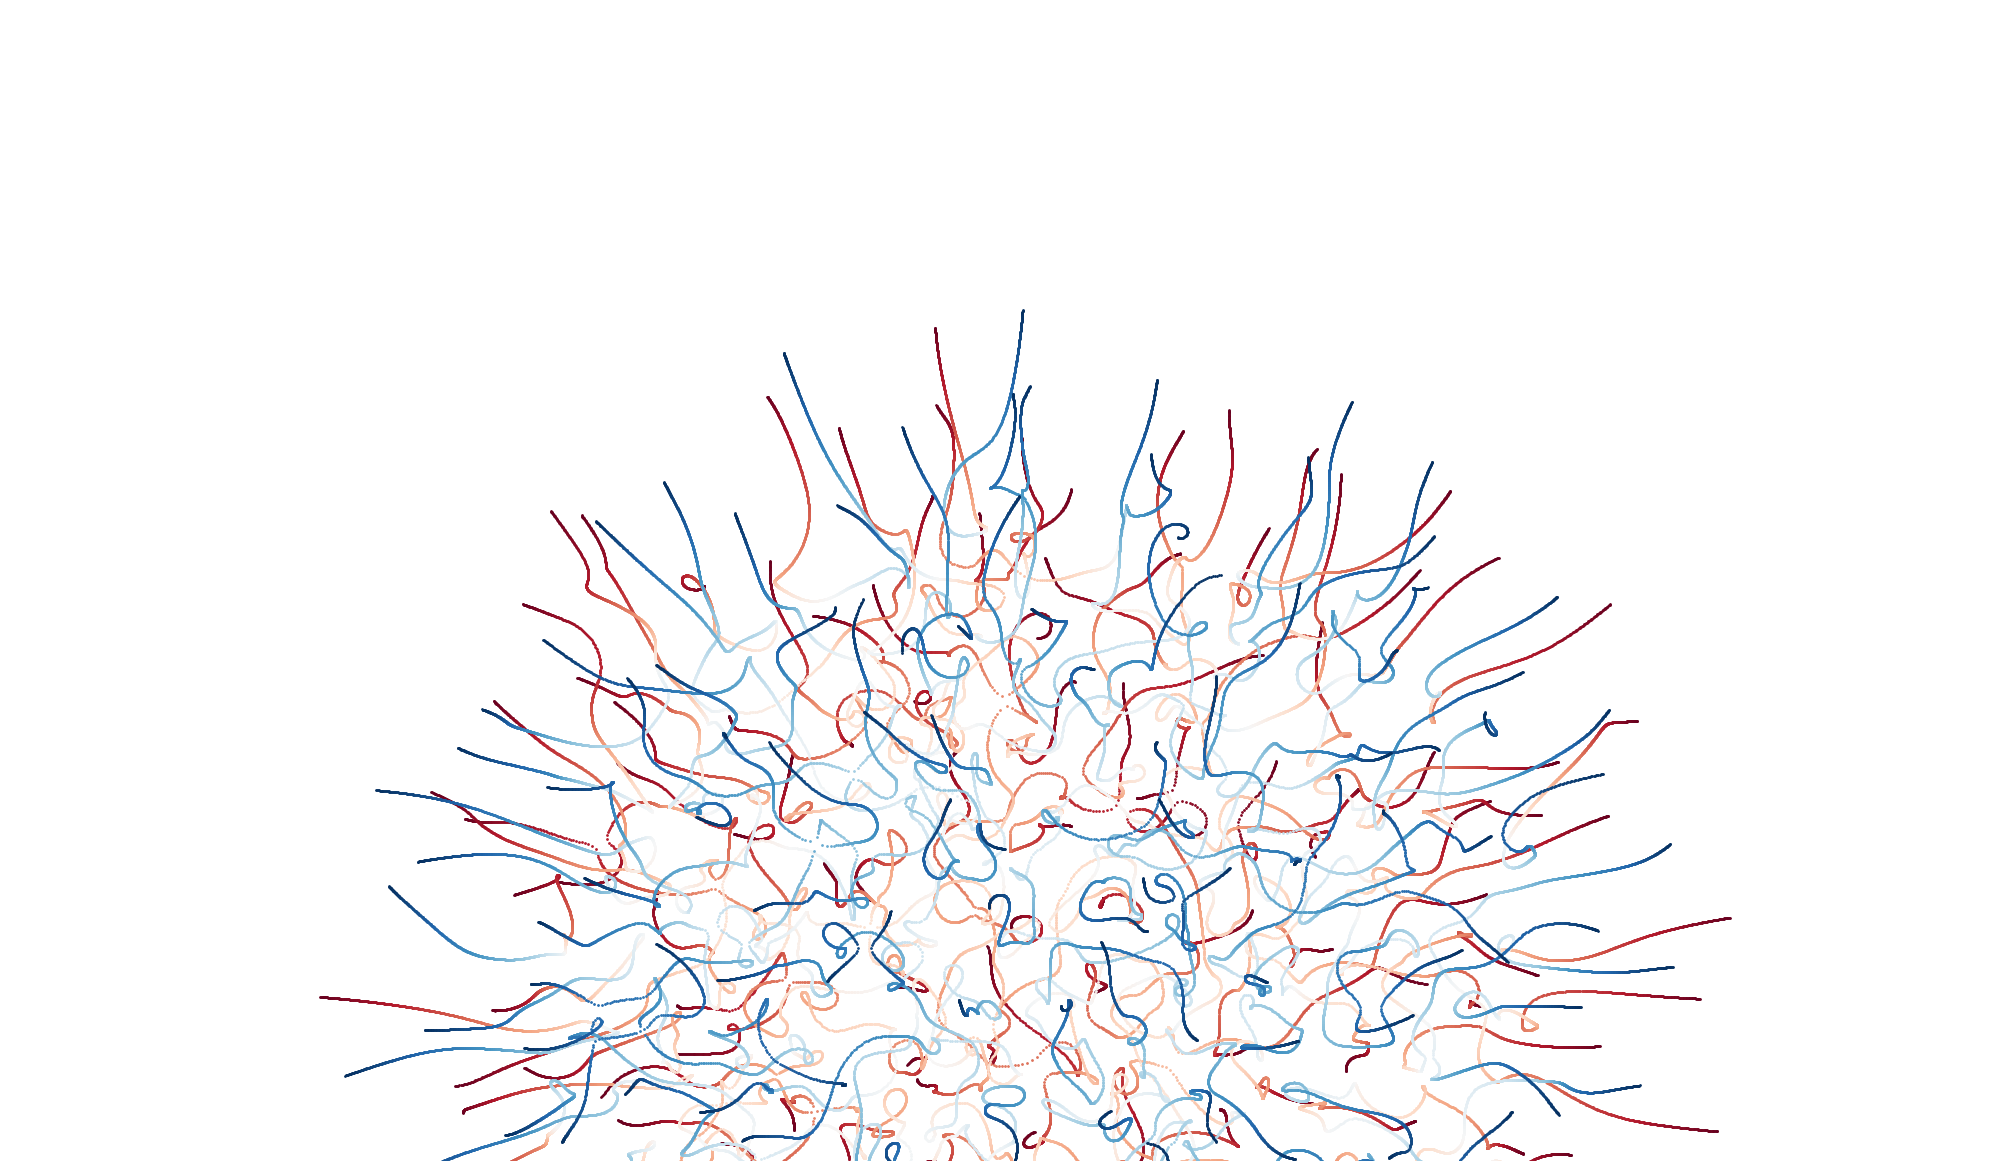
\includegraphics[width=1.5\paperwidth]{./media/aesthetics/croppedCircle.png}
		};
	\end{tikzpicture}
}{}
%------------

%TOC
\setbeamertemplate{section in toc}[sections numbered]
\setbeamertemplate{subsection in toc}[subsections numbered]
\setbeamerfont{subsection in toc}{size=\small, shape=\itshape}

%Templetae
\setbeamertemplate{navigation symbols}{}
\setbeamertemplate{note page}[compress]

%------------------------------------------------------------
%This block of code defines the information to appear in the
%Title page
\title[Asymptotics of Partition Functions of Coulomb Gases] %optional
{Asymptotics of Partition Functions of Coulomb Gases}

\subtitle{}

\author[João V. A. Pimenta] % (optional)
{João V. A. Pimenta\inst{1}}

\institute[ICMC] % (optional)
{
	\inst{1}%
	Insitituto de Ciências Matemáticas e de Computação - ICMC\\
	Universidade de São Paulo - USP
}

\date[Masters 2026] % (optional)
{Dissertation's defence for the degree of Master of Sciences in Mathematics. \\
Supervisor: Guilherme Silva}

\titlegraphic{
\includegraphics[height=1cm]{media/aesthetics/icmclogonb}}

%End of title page configuration block
%------------------------------------------------------------

%------------------------------------------------------------
%The next block of commands puts the table of contents at the 
%beginning of each section and highlights the current section:

\AtBeginSection[]{
	\begin{frame}
		\vfill
		\centering
		\includesvg[inkscapelatex=true, width=0.3\textwidth]{\secimage}
%		\begin{tikzpicture}
%		\begin{axis}[axis line style={opacity=0}, ticks=none,
%			xmin=-1.5, xmax=1.5,
%			ymin=-1.5, ymax=1.5,
%			xticklabel=\empty,
%			yticklabel=\empty,
%			xlabel={t = 0},
%			ylabel={a = 2},
%			xticklabel pos=top,
%			scatter/classes={%
%				a={ mark size=0.5pt}}
%			]
%			\addplot[skip coords between index={50}{500}, opacity=1, scatter, mark=x, black, only marks] table [col sep=comma] {\secimage};
%			\addplot[opacity=0.05, scatter, mark=*,draw opacity=0,black, only marks] table [col sep=comma] {\secimage};
%		\end{axis}
%		\end{tikzpicture}
		\begin{beamercolorbox}[sep=8pt,center,shadow=true,rounded=true]{title}
			\usebeamerfont{title}\insertsectionhead\par%
		\end{beamercolorbox}
		\vfill 
	\end{frame}
}

%------------------------------------------------------------
\definecolor{titleideablock}{HTML}{014508}
\definecolor{historycolor}{HTML}{b36630}
\definecolor{preamblecolor}{HTML}{d97836}



\newenvironment{ideablock}[1]{%
	\setbeamercolor{block title}{bg=titleideablock}
	\begin{block}{#1}}{\end{block}}

\newenvironment{history}[1]{%
	\setbeamercolor{block title}{bg=historycolor}
	\begin{block}{#1}}{\end{block}}
%------------------------------------------------------------

%------------------------------------------------------------
% math when ellipsis
%------------------------------------------------------------
\newcommand{\many}[2]{$#1_1, #1_2, \dots, #1_#2$}
\newcommand{\cmany}[3]{$#1_1 #3 #1_2 #3 \dots #3 #1_#2$}
\newcommand{\mmany}[2]{ #1_1, #1_2, \dots, #1_#2 }
\newcommand{\mcmany}[3]{#1_1 #3 #1_2 #3 \dots #3 #1_#2}


%-----------------------------------------------------------
% polynomials and such
%------------------------------------------------------------
%Hermite
\newcommand{\He}{\mathrm{He}} 
%Hermite Polynomials
\newcommand{\Het}{\tilde{\mathrm{H}}} 
%Hermite Polynomials
\newcommand{\Her}{\mathrm{H}} 
% Airy Kernel
\DeclareMathOperator{\Ai}{Ai}
% sine Kernel
\newcommand{\Sine}{\mathcal{S}}
% weight function
\newcommand{\wf}{w}
% pffafian
\DeclareMathOperator{\pf}{\text{Pf}}
% potential
\newcommand{\V}{V}
\newcommand{\Q}{Q}
%interacteing coulomb kernel
\newcommand{\g}{\mathfrak{g}}

\DeclareMathOperator{\cpct}{cap}

%------------------------------------------------------------
% \e ensemble
%------------------------------------------------------------
% matrices
\newcommand{\m}[1]{\hat#1} 
%
\newcommand{\spec}[1]{\text{spec}\{\hat{#1}\}}
% ensemble
\newcommand{\eE}{\mathcal{E}} 
% ensemble set
\newcommand{\eS}{\mathcal{S}} 
%  ensemble measure
\newcommand{\eP}{\mathcal{P}}
% eigenvalue measure
\newcommand{\pe}{\mu} 
% scaled eigenvalue
\newcommand{\Spe}{\tilde{\mathfrak{p}}}  
% measure in 
\newcommand{\p}{\mathtt{p}} 
% scaled eigenvalues measure
\newcommand{\Sp}{\tilde{\mathtt{p}}} 
%partition function
\newcommand{\pZ}[2]{\mathcal{Z}_{#1}^{#2}} 
%partition function
\newcommand{\pN}[2]{\mathcal{N}_{#1}^{#2}} 
% 
\newcommand{\Hf}{\mathcal{H}}

%------------------------------------------------------------
% math
%------------------------------------------------------------
%
\newcommand{\n}{\mathfrak{n}}
\newcommand{\normL}[3]{||#2||_{L^#1 #3}}
% support for function
\DeclareMathOperator{\supp}{supp}
\DeclareMathOperator{\sgn}{sgn}
%\DeclareMathOperator{\pv}{P.V.}
\DeclareMathOperator{\Ct}{\mathcal{C}}
% Genereric Field
\newcommand{\F}{\mathbb{F}}
% Generic Set
\newcommand{\Se}{\mathbb{S}}
% Variance
\DeclareMathOperator{\Var}{\mathbb{V}ar}
% volume
\DeclareMathOperator{\vol}{Vol}
% Jacobian
\newcommand{\J}{J}
\newcommand{\Hh}{\mathbb{H}}
% ceiling and floor funcitons
\DeclarePairedDelimiter\ceil{\lceil}{\rceil}
\DeclarePairedDelimiter\floor{\lfloor}{\rfloor}
% order function
\newcommand{\boh}{\mathit{o}}
\newcommand{\Boh}{\mathcal{O}}
% symbols with underscrips
\newcommand\underrel[2]{\mathrel{\mathop{#2}\limits_{#1}}}
%set notation
\newcommand{\set}[1]{\{#1\}}
% conjugate notation
\newcommand{\cjgt}[1]{\overline{#1}}
% diagonal notation
\DeclareMathOperator{\diag}{diag}
% trace operator
%\DeclareMathOperator{\tr}{Tr}
% sign operator
\DeclareMathOperator{\sign}{sign}
% real part
\DeclareMathOperator{\re}{Re}
% imaginary part
\DeclareMathOperator{\im}{Im}
\renewcommand{\Im}{\mathop{\textrm Im}}
% diff operator
\DeclareMathOperator{\Df}{D}
%\newcommand{\dd}{\mathrm{d}}
% neperian number
\DeclareMathOperator{\ee}{e}
% imaginary number
\newcommand{\ii}{\mathrm{i}}
% Identity
\newcommand{\Id}{\vmathbb{1}}
% indicator
\newcommand{\Ind}{\vmathbb{1}}
% Set of numbers
\newcommand{\N}{\mathbb{N}}
\newcommand{\C}{\mathbb{C}}
\newcommand{\R}{\mathbb{R}}
\newcommand{\Z}{\mathbb{Z}}
\newcommand{\Hq}{\mathbb{H}}
\newcommand{\M}{\mathcal{M}}
% Expectation
\DeclareMathOperator{\E}{\mathbb{E}}
\DeclareMathOperator{\res}{Res}

% Defintions
\newcommand*{\deff}{\mathrel{\vcenter{\baselineskip0.5ex \lineskiplimit0pt
			\hbox{\scriptsize.}\hbox{\scriptsize.}}}%
	=}
\newcommand*{\revdeff}{=\mathrel{\vcenter{\baselineskip0.5ex \lineskiplimit0pt
			\hbox{\scriptsize.}\hbox{\scriptsize.}}}%
}

% MATH DECLARATION
\numberwithin{equation}{section} %numeracao dentro de secoes

\def\eigenvalues{\tikz[baseline=3ex, scale=0.3]{
			\begin{axis}[axis line style={opacity=1}, ticks=none,
			xmin=-1.25, xmax=1.25,
			ymin=-1.25, ymax=1.25,
			axis x line=middle,
			axis y line=middle,
			xticklabel=\empty,
			yticklabel=\empty,
			xticklabel pos=top,
			xlabel=$\R$,
			ylabel=$\ii$,
			scatter/classes={%
				a={ mark size=0.5}}
			]
			\addplot[skip coords between index={100}{500}, opacity=1, scatter, mark=x, black, only marks] table [col sep=comma] {./media/aesthetics/5lines/a2t0.csv};
			\end{axis}
		}
}

\def\eigenvaluesfar{\tikz[baseline=5ex, scale=0.5]{
		\begin{axis}[axis line style={opacity=1}, ticks=none,
			xmin=-1.5, xmax=1.5,
			ymin=-1.5, ymax=1.5,
			axis x line=middle,
			axis y line=middle,
			xticklabel=\empty,
			yticklabel=\empty,
			xticklabel pos=top,
			xlabel=$\R$,
			ylabel=$\ii$,
			scatter/classes={%
				a={ mark size=0.5}}
			]
			\addplot[skip coords between index={50}{500}, opacity=1, scatter, mark=x, black, only marks] table [col sep=comma] {./media/aesthetics/times2.csv};
		\end{axis}
	}
}

\def\eigenvaluesclose{\tikz[baseline=5ex, scale=0.5]{
		\begin{axis}[axis line style={opacity=1}, ticks=none,
			xmin=-1.5, xmax=1.5,
			ymin=-1.5, ymax=1.5,
			axis x line=middle,
			axis y line=middle,
			xticklabel=\empty,
			yticklabel=\empty,
			xticklabel pos=top,
			xlabel=$\R$,
			ylabel=$\ii$,
			scatter/classes={%
				a={ mark size=0.5}}
			]
			\addplot[skip coords between index={50}{500}, opacity=1, scatter, mark=x, black, only marks] table [col sep=comma] {./media/aesthetics/times05.csv};
		\end{axis}
	}
}

\usepackage[dvipsnames]{xcolor}

\newenvironment{colorblock}[2]{%
	\setbeamercolor{block title}{#2}
	\begin{block}{#1}}{\end{block}}
	

\newcommand{\secimage}{./media/aesthetics/S1}

\begin{document}

%The next statement creates the title page.
\frame{\titlepage}

%---------------------------------------------------------
%This block of code is for the table of contents after
%the title page
{
%\usebackgroundtemplate{
\includegraphics[width=\paperwidth]{./media/aesthetics/AstecDiamond.png}}
\begin{frame}
\frametitle{Table of Contents}
\tableofcontents
\end{frame}
}

\section{Random Matrices}

\subsection{Why is a Random Matrix}

%\begin{frame}
%%	\begin{columns}
%%		\begin{column}{0.5\textwidth}
%%			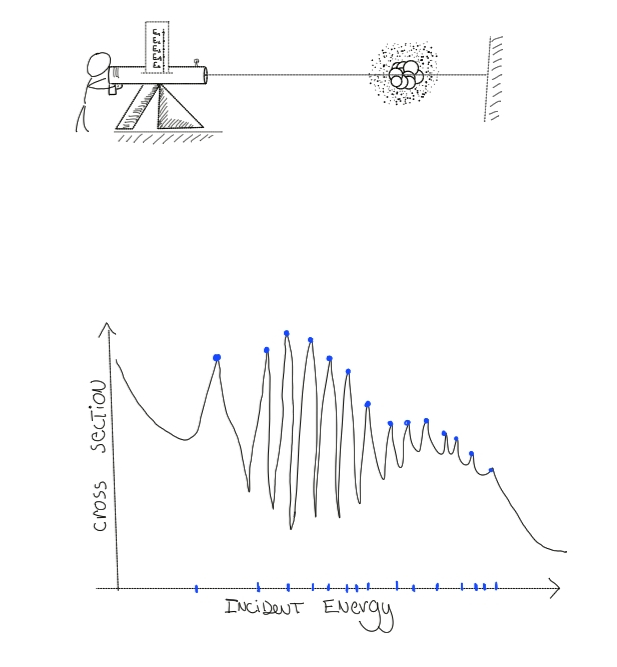
\includegraphics[width=\textwidth]{./media/aesthetics/nuclearscattering.jpg}
%%		\end{column}
%%		\visible<2-3>{
%%			\begin{column}{0.5\textwidth} 
%%				\vspace{1cm}
%%				\begin{equation*}
%%					\Hf \phi_i = E_i \phi_i
%%				\end{equation*}
%%				\visible<3>{
%%					\hspace{0.1cm}
%%					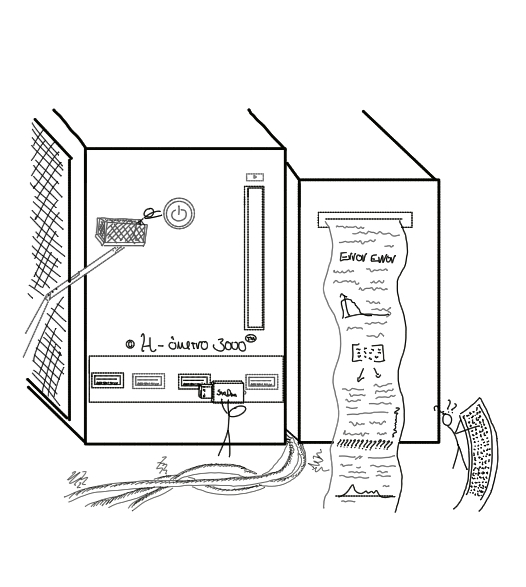
\includegraphics[width=0.8\textwidth]{./media/aesthetics/computer.jpg}
%%				}
%%			\end{column}
%%		}
%%	\end{columns}	
%%	
%\end{frame}

%\begin{frame}
%	\begin{block}{Eugene Wigner - \textit{On the Wigner Surmise} (1956)}
%		``\textit{Perhaps I am now too courageous when I try to guess the distribution of the distances between successive levels (of energies of heavy nuclei) [...] The question is simply what are the distances of the characteristic values of a symmetric matrix with random coefficients.}''
%	\end{block}
%	\vspace{5.5cm}
%	\visible<2-3>{
%		\begin{columns}
%			\begin{column}{0.25\textwidth} 
%				\visible<3>{
%					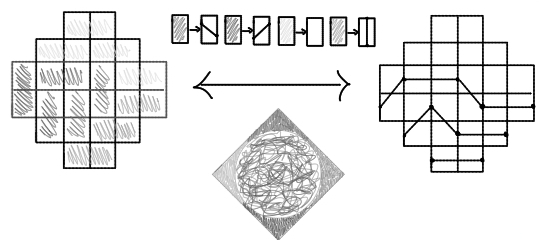
\includegraphics[width=\textwidth]{./media/aesthetics/aztecdiamond.jpg}
%					
%					
\includegraphics[width=\textwidth]{./media/aesthetics/matching.jpg}
%				}
%			\end{column}
%			\begin{column}{0.5\textwidth}
%				\hspace{0.2cm}
%				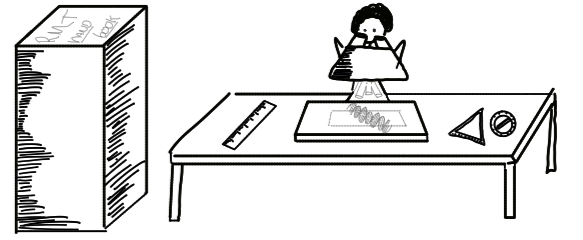
\includegraphics[width=0.9\textwidth]{./media/aesthetics/modelling.jpg}
%			\end{column}
%			\begin{column}{0.25\textwidth} 
%				\visible<3>{
%					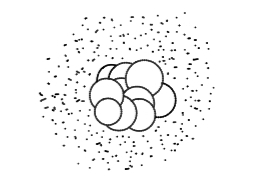
\includegraphics[width=0.8\textwidth]{./media/aesthetics/nucleii.jpg}
%					
%					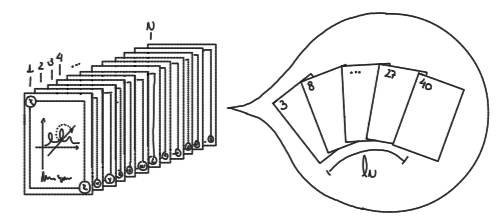
\includegraphics[width=\textwidth]{./media/aesthetics/sequences.jpg}
%				}
%			\end{column}
%		\end{columns}
%	}	
%\end{frame}

{
	\setbeamercolor{background canvas}{bg=}
	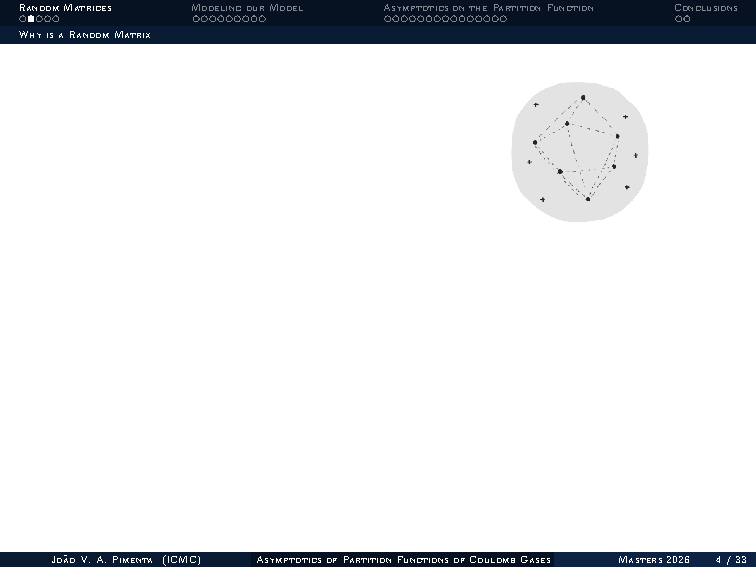
\includepdf[pages={1-}]{why.pdf}
}

\addtocounter{framenumber}{+1}

\subsection{What is a Random Matrix}

\begin{frame}
	\vspace{-0.5cm}
	\only<8->{
		We can think of the matrix itself as a random variable, a measurable map from a probability measure space to $\mathcal{M}_n$.
		\vspace{-0.7cm}
	}
	\only<1-2>{\vspace{-0.25cm}}
	\only<1-7>{
	A \textit{random matrix} is a matrix with \textit{random variables} as entries. 
	}
	\vfill
	\begin{columns}
		\begin{column}{0.5\textwidth}
			\only<1,2>{
				\begin{center}
					$
					\begin{bmatrix}
						x_{1,1} & x_{1,2}& x_{1,3} & x_{1,4}  \\
						x_{2,1} & x_{2,2}& x_{2,3} & x_{2,4} \\
						x_{3,1} & x_{3,2}& x_{3,3} & x_{3,4}  \\
						x_{4,1} & x_{4,2}& x_{4,3} & x_{4,4}  \\
						x_{5,1} & x_{5,2}& x_{5,3} & x_{5,4}
					\end{bmatrix}
					$
				\end{center}
			}
			\only<3>{
				\begin{center}
					$
					\begin{bmatrix}
						-1 & -1 & 1 & 1 \\
						-1 & 1 & -1 & 1 \\
						-1 & 1 & -1 & -1 \\
						-1 & -1 & 1 & -1 \\
						-1 & 1 & -1 & 1 
					\end{bmatrix}
					$
										\vspace{0.5cm}
				\end{center}
			}
			\only<4>{
				\begin{center}
					$
					\begin{bmatrix}
						0.213&0.368&0.912&0.881\\
						0.759&0.692&0.000&0.332\\
						0.898&0.987&0.422&0.623\\
						0.145&0.880&0.522&0.686\\
						0.753&0.687&0.787&0.515
					\end{bmatrix}
					$
										\vspace{0.5cm}
				\end{center}
			}
			\only<5>{
				\begin{center}
					$
					\begin{bmatrix}
						-0.022&-1.340&-0.483&-1.134\\
						1.752&-1.644&1.081&-0.936\\
						-1.058&-0.091&0.544&-0.382\\
						0.633&0.567&0.606&-0.621\\
						-0.316&-1.128&-0.150&0.251
					\end{bmatrix}
					$
					\vspace{0.5cm}
				\end{center}
			}
			\only<6>{
			\begin{center}
				$
				\left[\begin{smallmatrix}
					-2.0+0.1\ii&-0.2-0.9\ii&-0.4-0.3\ii&-0.3+1.0\ii\\
					-1.6-0.8\ii&0.3-0.6\ii&-1.7+0.9\ii&-0.1+0.3\ii\\
					-0.5-0.9\ii&-0.5+0.2\ii&1.2+1.0\ii&0.4-1.3\ii\\
					-0.6+2.4\ii&0.1-0.7\ii&-0.2+1.6\ii&0.6-0.4\ii\\
					0.1-1.3\ii&-0.2-0.9\ii&1.2-1.6\ii&2.1+2.0\ii\\
				\end{smallmatrix}\right]
				$
				\vspace{0.8cm}
			\end{center}
			}
			\only<7-9>{
				\begin{center}
					$
					\left[\begin{smallmatrix}
					-0.8&-0.2-1.5\ii&0.9-0.6\ii&-3.2+2.3\ii \\
					-0.2+1.5\ii&0.5&-1.8-0.8\ii&1.5+1.8\ii \\
					0.9+0.6\ii&-1.8+0.8\ii&1.8&2.1+2.5\ii \\
					-3.2-2.3\ii&1.5-1.8\ii&2.1-2.5\ii&2.4
					\end{smallmatrix}\right]
					$
					\vspace{0.8cm}
				\end{center}
			}
		\end{column}
		\begin{column}{0.5\textwidth}  %%<--- here
			\only<1>{
			\begin{table}
				\centering
				\begin{tabular}{l | c | c }
					$\p(x_{i,j})$ & $\Se$ & $\M_n$ \\
					\hline \hline
					Discrete& $\R$  & General\\ 
					Uniform & $\C$ &  Hermitian \\
					Gaussian & $\mathbb{H}$ & Normal \\
					\vdots  & \vdots  &  \vdots \\
					\hline
				\end{tabular}
			\end{table}
			}
			\only<2>{
				\begin{table}
					\centering
					\begin{tabular}{l | c | c }
						$\p(x_{i,j})$ & $\Se$ & $\M_n$ \\
						\hline \hline
						Discrete& \cellcolor{red!10}$\R$  & \cellcolor{green!10}General\\ 
						Uniform & $\C$ &  Hermitian \\
						Gaussian & $\mathbb{H}$ & Normal \\
						\vdots  & \vdots  &  \vdots \\
						\hline
					\end{tabular}
				\end{table}
			}
			\only<3>{
				\begin{table}
					\centering
					\begin{tabular}{l | c | c }
						$\p(x_{i,j})$ & $\Se$ & $\M_n$ \\
						\hline \hline
						\cellcolor{blue!10} Discrete& \cellcolor{red!10}$\R$  & \cellcolor{green!10}General\\ 
						Uniform & $\C$ &  Hermitian \\
						Gaussian & $\mathbb{H}$ & Normal \\
						\vdots  & \vdots  &  \vdots \\
						\hline
						\multicolumn{3}{c}{	\fcolorbox{white}{blue!10}{} \!\!\!\! \fcolorbox{white}{red!10}{}  \!\!\!\! \fcolorbox{white}{green!10}{}}
					\end{tabular}
				\end{table}
			}
			\only<4>{
				\begin{table}
					\centering
					\begin{tabular}{l | c | c }
						$\p(x_{i,j})$ & $\Se$ & $\M_n$ \\
						\hline \hline
						Discrete& \cellcolor{red!10}$\R$  & \cellcolor{green!10}General\\ 
						\cellcolor{blue!10}Uniform & $\C$ &  Hermitian \\
						Gaussian & $\mathbb{H}$ & Normal \\
						\vdots  & \vdots  &  \vdots \\
						\hline
						\multicolumn{3}{c}{	\fcolorbox{white}{blue!10}{} \!\!\!\! \fcolorbox{white}{red!10}{}  \!\!\!\! \fcolorbox{white}{green!10}{}} \\
					\end{tabular}
				\end{table}
			}
			\only<5>{
				\begin{table}
					\centering
					\begin{tabular}{l | c | c }
						$\p(x_{i,j})$ & $\Se$ & $\M_n$ \\
						\hline \hline
						Discrete& \cellcolor{red!10}$\R$  & \cellcolor{green!10}General\\ 
						Uniform & $\C$ &  Hermitian \\
						\cellcolor{blue!10}Gaussian & $\mathbb{H}$ & Normal \\
						\vdots  & \vdots  &  \vdots \\
						\hline
						\multicolumn{3}{c}{	\fcolorbox{white}{blue!10}{} \!\!\!\! \fcolorbox{white}{red!10}{}  \!\!\!\! \fcolorbox{white}{green!10}{}} \\
						\multicolumn{3}{c}{ 
							Ginibre Orthogonal Ensemble} 
					\end{tabular}
				\end{table}
			}
			\only<6>{
				\begin{table}
					\centering
					\begin{tabular}{l | c | c }
						$\p(x_{i,j})$ & $\Se$ & $\M_n$ \\
						\hline \hline
						Discrete& $\R$  & \cellcolor{green!10}General\\ 
						Uniform & \cellcolor{red!10}$\C$ &  Hermitian \\
						\cellcolor{blue!10}Gaussian & $\mathbb{H}$ & Normal \\
						\vdots  & \vdots  &  \vdots \\
						\hline
						\multicolumn{3}{c}{	\fcolorbox{white}{blue!10}{} \!\!\!\! \fcolorbox{white}{red!10}{}  \!\!\!\! \fcolorbox{white}{green!10}{}} \\
						\multicolumn{3}{c}{ 
							Ginibre Unitary Ensemble} 
					\end{tabular}
				\end{table}
			}
			\only<7-8>{
				\begin{table}
					\centering
					\begin{tabular}{l | c | c }
						$\p(x_{i,j})$ & $\Se$ & $\M_n$ \\
						\hline \hline
						Discrete& $\R$  & General\\ 
						Uniform & \cellcolor{red!10}$\C$ &  \cellcolor{green!10}Hermitian \\
						\cellcolor{blue!10}Gaussian & $\mathbb{H}$ & Normal \\
						\vdots  & \vdots  &  \vdots \\
						\hline
						\multicolumn{3}{c}{	\fcolorbox{white}{blue!10}{} \!\!\!\! \fcolorbox{white}{red!10}{}  \!\!\!\! \fcolorbox{white}{green!10}{}} \\
						\multicolumn{3}{c}{ 
							Gaussian Unitary Ensemble} 
					\end{tabular}
				\end{table}
			}
			\only<9>{
			\vspace{-0.15cm}
				\begin{table}
					\centering
					\begin{tabular}{l | c | c }
						$\eP(\m{X})$ & $\Se$ & $\M_n$ \\
						\hline \hline
						\cellcolor{blue!10}$\ee^{-n \tr(\m{X}^2)}$ &$\R$  & General\\ 
						$\ee^{-n \tr{(\m{X}^* \m{X})}}$ &  \cellcolor{red!10}$\C$ &  \cellcolor{green!10}Hermitian \\
						$\ee^{-n \tr{(Q(\m{X}))}}$ & $\mathbb{H}$ & Normal \\
						\vdots  & \vdots  &  \vdots \\
						\hline
						\multicolumn{3}{c}{	\fcolorbox{white}{blue!10}{} \!\!\!\! \fcolorbox{white}{red!10}{}  \!\!\!\! \fcolorbox{white}{green!10}{}} \\
						\multicolumn{3}{c}{Gaussian Unitary Ensemble} 
					\end{tabular}
				\end{table}
			\vspace{-0.15cm}
			}
		\end{column}
	\end{columns}
	\vfill
	\only<1-3>{
		\visible<3>{
		\begin{equation*}
			\eP(\m{X}) = \prod_{i,j=1}^{n} p(x_{i,j}) = U^{n^2}(\{-1, 1\})
		\end{equation*}
		}
    }
	\only<4>{
		\begin{equation*}
			\eP(\m{X}) = \prod_{i,j=1}^{n} p(x_{i,j}) = U^{n^2}([0,1])
		\end{equation*}
	}
	\only<5>{
		\begin{equation*}
			\eP(\m{X}) = \prod_{i,j=1}^{n} \ee^{-n x_{i,j}^2}
		\end{equation*}
	}
	\only<6>{
		\begin{equation*}
			\eP(\m{X}) = \prod_{i,j=1}^{n} \ee^{-n x_{i,j}^2} \ee^{-n y_{i,j}^2}
		\end{equation*}
	}
	\only<7-8>{
		\begin{equation*}
			\eP(\m{X}) = \prod_{i=1}^{n} \ee^{-n z_{i,j}^2} \prod_{i>j}^{n} \ee^{-2n |z_{i,j}|^2}
		\end{equation*}
	}
	\only<9>{
		\begin{equation*}
			\eP(\m{X}) = \prod_{i=1}^{n} \ee^{-n z_{i,j}^2} \prod_{i>j}^{n} \ee^{-2n |z_{i,j}|^2} \propto \ee^{-n \tr(\m{X}^2)}
		\end{equation*}
	}
\end{frame}

\subsection{Normal Matrix Density}

\begin{frame}
	\only<1->{\vspace{0.1cm}}
	\only<1->{
	We can think of the matrix itself as a random variable, a measurable map from a probability measure space to $\mathcal{M}_n$.
	}
	\begin{columns}
		\begin{column}{0.5\textwidth}
		\only<2-3>{
			Normal matrices are similar to diagonal matrices, i.e.
			\begin{equation*}
				\m{X} = \m{U} \m{\Lambda} \m{U}^*.
			\end{equation*}
			Moreover, the spectra is typically simple. 
		}
		\only<4->{
			Invariance by unitary conjugation means independence of coordinates. 
			\begin{equation*}
				\dd\eP(\m{X}_1) = \dd\eP(\m{X}_2) \iff \m{X}_1 = \m{U} \m{X}_2 \m{U}^*
			\end{equation*}
			for some unitary $U$.
		}
		\end{column}
		\begin{column}{0.5\textwidth}  %%<--- here
		\only<1-5>{
			\begin{table}
				\centering
				\begin{tabular}{l | c | c }
					$\eP(\m{X})$ & $\Se$ & $\M_n$ \\
					\hline \hline
					$\ee^{-n \tr(\m{X}^2)}$ &$\R$  & General\\ 
					$\ee^{-n \tr{(\m{X}^* \m{X})}}$ &  \cellcolor{red!10}$\C$ &  Hermitian \\
					$\ee^{-n \tr{(Q(\m{X}))}}$ & $\mathbb{H}$ & \cellcolor{green!10}Normal \\
					\vdots  & \vdots  &  \vdots \\
					\hline
					\multicolumn{3}{c}{ \fcolorbox{white}{red!10}{}  \!\!\!\! \fcolorbox{white}{green!10}{}} \\
				\end{tabular}
			\end{table}
		}
		\only<6->{
			\begin{table}
				\centering
				\begin{tabular}{l | c | c }
					$\eP(\m{X})$ & $\Se$ & $\M_n$ \\
					\hline \hline
					$\ee^{-n \tr(\m{X}^2)}$ &$\R$  & General\\ 
					$\ee^{-n \tr{(\m{X}^* \m{X})}}$ &  \cellcolor{red!10}$\C$ &  Hermitian \\
					\cellcolor{blue!10}$\ee^{-n \tr{(Q(\m{X}))}}$ & $\mathbb{H}$ & \cellcolor{green!10}Normal \\
					\vdots  & \vdots  &  \vdots \\
					\hline
					\multicolumn{3}{c}{	\fcolorbox{white}{blue!10}{} \!\!\!\! \fcolorbox{white}{red!10}{}  \!\!\!\! \fcolorbox{white}{green!10}{}} \\
				\end{tabular}
			\end{table}
		}
		\end{column}
	\end{columns}
	\visible<2->{
		\only<5->{
			We want that $\dd \eP(\m{X}) = \eP(\m{X}) \dd \m{X}$ is invariant.
		}
		\only<1-2>{
			\vspace{3.27cm}
		}
		\only<5,6>{
			\vspace{2.8cm}
		}
		\only<3-4>{
			\begin{equation*}
				\m{X} \mapsto (\m{\Lambda}, \m{U}) = \left(
					\begin{tikzpicture}[baseline=8ex, scale=0.70]
					\begin{axis}[axis line style={opacity=1}, ticks=none,
						xmin=-1.5, xmax=1.5,
						ymin=-1.5, ymax=1.5,
						axis x line=middle,
						axis y line=middle,
						xticklabel=\empty,
						yticklabel=\empty,
						xticklabel pos=top,
						xlabel=$\R$,
						ylabel=$\ii \R$,
						scatter/classes={%
							a={ mark size=0.5pt}}
						]
						\addplot[skip coords between index={10}{500}, opacity=1, scatter, mark=x, black, only marks] table [col sep=comma] {./media/aesthetics/5lines/a2t0.csv};
					\end{axis}
				\end{tikzpicture} \hspace{0.3cm},
				\begin{tikzpicture}[baseline=0ex, line cap=round]
					\coordinate (O) at (0,0);
					\coordinate (A) at ( -5:1.1);
					\coordinate (B) at ( 55:1.4);
					\coordinate (C) at (130:1.2);
					\coordinate (D) at (210:2.0);
					\coordinate (E) at (65:1.60);
					\coordinate (F) at (-110:1.2);
					\coordinate (G) at (30:1.3);
					\coordinate (H) at (200:1.2);
					\coordinate (I) at (-30:1.4);
					\coordinate (J) at (123:0.4);
					\draw[vector,black] (O) -- (A) node[right=-2] {};
					\draw[vector,black] (O) -- (B) node[above right=-3] {};
					\draw[vector,black] (O) -- (C) node[above left=-3] {};
					\draw[vector,black] (O) -- (D) node[left=-1] {};
					\draw[vector,black] (O) -- (E) node[left=-1] {};
					\draw[vector,black] (O) -- (F) node[left=-1] {};
					\draw[vector,black] (O) -- (G) node[left=-1] {};
					\draw[vector,black] (O) -- (H) node[left=-1] {};
					\draw[vector,black] (O) -- (I) node[left=-1] {};
					\draw[vector,black] (O) -- (J) node[left=-1] {};
				\end{tikzpicture} \hspace{-1cm}
				\right)
			\end{equation*}
%	\begin{columns}
%		\begin{column}{0.1\textwidth}  %%<--- here
%			\begin{center}
%				$ \m{X} \mapsto
%				$
%			\end{center}
%		\end{column}
%		\begin{column}{0.4\textwidth}  %%<--- here
%			\begin{center}
%				\begin{tikzpicture}[scale=0.70]
%					\begin{axis}[axis line style={opacity=1}, ticks=none,
%						xmin=-1.5, xmax=1.5,
%						ymin=-1.5, ymax=1.5,
%						axis x line=middle,
%						axis y line=middle,
%						xticklabel=\empty,
%						yticklabel=\empty,
%						xticklabel pos=top,
%						xlabel=$\R$,
%						ylabel=$\ii \R$,
%						scatter/classes={%
%							a={ mark size=0.5pt}}
%						]
%						\addplot[skip coords between index={10}{500}, opacity=1, scatter, mark=x, black, only marks] table [col sep=comma] {./media/aesthetics/5lines/a2t0.csv};
%					\end{axis}
%				\end{tikzpicture}
%			\end{center}
%		\end{column}
%		\begin{column}{0.4\textwidth}
%			\begin{center}
%				\begin{tikzpicture}[line cap=round]
%					\coordinate (O) at (0,0);
%					\coordinate (A) at ( -5:1.1);
%					\coordinate (B) at ( 55:1.4);
%					\coordinate (C) at (130:1.2);
%					\coordinate (D) at (210:2.0);
%					\coordinate (E) at (65:1.60);
%					\coordinate (F) at (-110:1.2);
%					\coordinate (G) at (30:1.3);
%					\coordinate (H) at (200:1.2);
%					\coordinate (I) at (-30:1.4);
%					\coordinate (J) at (123:0.4);
%					\draw[vector,black] (O) -- (A) node[right=-2] {};
%					\draw[vector,black] (O) -- (B) node[above right=-3] {};
%					\draw[vector,black] (O) -- (C) node[above left=-3] {};
%					\draw[vector,black] (O) -- (D) node[left=-1] {};
%					\draw[vector,black] (O) -- (E) node[left=-1] {};
%					\draw[vector,black] (O) -- (F) node[left=-1] {};
%					\draw[vector,black] (O) -- (G) node[left=-1] {};
%					\draw[vector,black] (O) -- (H) node[left=-1] {};
%					\draw[vector,black] (O) -- (I) node[left=-1] {};
%					\draw[vector,black] (O) -- (J) node[left=-1] {};
%				\end{tikzpicture}
%			\end{center}
%		\end{column}
%	\end{columns}
		}
	\only<7>{
	\vspace{0.1cm}
	\begin{align*}
		\exp\left(-n\tr{Q(\m{U}\m{X_1}\m{U}^*)}\right) &= \exp\left(-n\tr{Q(\m{U}^*\m{U}\m{X_1})}\right) = \exp\left(-n\tr{Q(\m{X_1})}\right) \\ & = \exp\left(-n\tr{Q(\m{U}\m{\Lambda}\m{U}^*)}\right) = \exp\left(-n\sum_i^n {Q(\lambda_i)} \right).
	\end{align*}
	\vspace{0.1cm}
	}
	\only<8>{
	\begin{equation*}
		\dd \m{X} = \prod_{1 \leq i < j \leq n} |z_i - z_j|^2 \prod_{i=1}^{n} \dd^2 z_i  \dd \m{U} ,
	\end{equation*}
	where $\dd \m{U}$ is the Haar measure on eigenvectors and $\dd^2 z$ is Lebesgue measure on $\C$.
	\vspace{0.5cm}
	}
	}
\end{frame}

%\begin{frame}
%	\begin{theorem}	
%	\label{Theorem: Weyls}
%	\textit{(Weyl's integration formula - Unitary case)} 
%	The measure $\dd \m{X}$ decomposes almost everywhere in $\mathcal{N}(\C)$ as 
%	\begin{equation*}
%		\dd \m{X} = \dd \m{U} \prod_{1 \leq i < j \leq n} |z_i - z_j|^2  \prod_{i=1}^{n} \dd^2 z_i,
%	\end{equation*}
%	where $\{z_i\}_{i=1}{n}$ is the spectrum of $\m{X}$, $\m{M} = \m{U} \m{\Lambda} \m{U}^*$ for $\m{\Lambda} =\diag\{z_i\}_{i=1}^n$, $\m{U} \in U(n)/U(1)^n$ and the measure
%	\begin{equation*}
%		\dd \m{U} = 2^{\frac{n(n-1)}{4}} \prod_{i<j} \dd^2 u_{i,j}, \quad \dd^2 u_{i,j} = (\m{U}^*)_{i,k}\dd^2\m{U}_{k,j}
%	\end{equation*}
%	on $U(n)/U(1)^n$ is induced by the measure on $U(n)$ and is a Haar measure.
%\end{theorem}
%\end{frame}

\begin{frame}
	We set the ensemble
	\begin{equation*}
		\eE = (\eS, \eP) \quad \text{with} \quad 
		\begin{cases}
			\eS = \mathcal{N}_n(\C) \\
			\eP(\m{X}) = \exp\left\{- n \tr(Q(\m{X}))\right\}
		\end{cases}
	\end{equation*}
	such that 
	\begin{equation*}
		\dd \eP(\m{X}) = \prod_ {i < j}^n |z_i - z_j|^2 \prod_{j=1}^{n} \ee^{- n \Q(z_j)} \dd^2 z_j \dd \m{U}.
	\end{equation*}
	\visible<2->{
	\begin{align*}
		\int_{\mathcal{M}_n} \dd \eP(\m{X}) & = \int_{\C^n} \int_{\tilde{U}(n)}  \prod_ {i < j}^n |z_i - z_j|^2 \prod_{j=1}^{n} \ee^{- n \Q(z_j)} \dd^2 z_j \dd \m{U} \\ & = \int_{\C^n} \frac{\prod_ {i < j}^n |z_i - z_j|^2 \prod_{j=1}^{n} \ee^{- n \Q(z_j)}}{\pZ{n}{Q}}  \dd^2 z_j
	\end{align*}
} \visible<3->{ we have
	\begin{equation*}
		p_n(\{z_i\}_{i=1}^n) = \frac{1}{\pZ{n}{Q}} \prod_ {i < j}^n |z_i - z_j|^2 \prod_{j=1}^{n} \ee^{- n \Q(z_j)} 
	\end{equation*}
}
\end{frame}
%---------------------------------------------------------




{
	\renewcommand{\secimage}{./media/aesthetics/S2}
	\section{Modeling our Model}
}

\subsection{Coulomb Gas}

\begin{frame}
	\only<5->{\vspace{0.39cm}}
	We know that
	\only<1-4>{
		\begin{equation*}
			p_n(\{z_i\}_{i=1}^n) = p\left( \eigenvalues \right) = \frac{1}{\pZ{n}{Q}} \prod_ {i < j}^n |z_i - z_j|^2 \prod_{j=1}^{n} \ee^{- n \Q(z_j)} 
		\end{equation*}
	}
	\only<1-4>{
		\visible<2-4>{
	We can notice two effects, one coming from the Jacobian and the other one from $Q$.	
		\begin{equation*}
			p_n\left( \eigenvalues \right) >
			\begin{cases}
				\visible<3->{
				p_n\left( \eigenvaluesclose \right), \quad \text{the interactions dominates.} \\
				\\
				}
				\visible<4>{
				p_n\left( \eigenvaluesfar \right), \quad \text{the external potential dominates$.^*$}
			}
			\end{cases}
	\end{equation*}
}
	}
	\only<5->{
		\vspace{0.159cm}
		\begin{align*}
			& p_n(\{z_i\}_{i=1}^n) = p\left( \eigenvalues \right) = \frac{1}{\pZ{n}{Q}} \prod_ {i < j}^n |z_i - z_j|^2 \prod_{j=1}^{n} \ee^{- n \Q(z_j)}  \\
			\visible<6->{& = \frac{1}{\pZ{n}{Q}} \exp\left\{- n^2 \left( \frac{1}{n} \sum_{i = 1}^{n} \Q(z_i) + \frac{1}{n^2} \sum_{i \neq j} \ln |z_i - z_j| \right) \right\} \\}
			\visible<7->{& = \frac{\ee^{-n^2 \Hf(\chi_n)}}{\pZ{n}{Q}}, \quad  \Hf(\chi_n) = \frac{1}{n} \sum_{i = 1}^{n} \Q(z_i) + \frac{1}{n^2} \sum_{i \neq j}^{n} \ln |z_i - z_j| }
		\end{align*}
		\visible<8->{The measure $\dd p_n$ models an Coulomb-interacting gas of charged indistinguishable particles under some external field $\Q$ on $\C$.}
		\vspace{1cm}
		
		\visible<9->{If we want to study this gases, how to describe its statistical properties?}
		\vspace{1.5cm}
	}
\end{frame}

\subsection{Point Process}

\begin{frame}{Point Process}
	\only<3-5>{
		\vspace{0.20cm}
	}
	Suppose there are $n$ particles at random locations in the complex plane $\C$ denoted by the configuration $\chi_n = \set{\mmany{z}{n}}$. 
	\begin{center}
	\vspace{-0.7cm}
	\begin{tikzpicture}
		\begin{axis}[axis line style={opacity=0}, ticks=none,
			xmin=-1.5, xmax=1.5,
			ymin=-1.5, ymax=1.5,
			xticklabel pos=top,
			scatter/classes={%
				a={ mark size=0.5pt}}
			]
			\addplot[skip coords between index={100}{500}, opacity=1, scatter, mark=x, black, only marks] table [col sep=comma] {./media/aesthetics/5lines/a2t0.csv};
			\only<3>{
			\draw[color = red] plot[smooth cycle] coordinates {(60,60) (85,100) (67,170) (120,150) (120,60)};
			}
			\only<4>{
			\draw[color = blue] plot[smooth cycle] coordinates {(160,200) (170,240) (150,260) (225,235) (280,200) (260, 180) (215, 200)};
			}
			\only<5>{
			\draw[color = teal] plot[smooth cycle] coordinates {(110,110) (100,160) (160,240) (135,155) (145,140)};
			}
		\end{axis}
	\end{tikzpicture}
	\vspace{-0.9cm}
	\end{center}	
	\visible<2->{Define a quantity \only<2,6->{$\xi(A)$}\only<3>{$\xi(\textcolor{red}{A_1})$}\only<4>{$\xi(\textcolor{blue}{A_2})$}\only<5>{$\xi(\textcolor{teal}{A_3})$} s.t.
	\begin{equation*}
		\only<2,6->{\xi(A)}\only<3>{\xi(\textcolor{red}{A_1})}\only<4>{\xi(\textcolor{blue}{A_2})}\only<5>{\xi(\textcolor{teal}{A_3})}=\sum_{k=1}^{n}\delta_{\only<3>{\textcolor{red}{A_1}}\only<4>{\textcolor{blue}{A_2}}\only<5>{\textcolor{teal}{A_3}}}(z_k)\only<3>{=\textcolor{red}{21}}\only<4>{=\textcolor{blue}{9}}\only<5>{=\textcolor{teal}{10}}
	\end{equation*}
	\visible<6->{
	This defines a \textit{random counting measure} in the usual sense. \visible<7->{A \textbf{point process} $\mathbb{P}$ on $\C$ is a probability measure on the space of all counting measures $\mathcal{N}(\C)$.}
	}
	}
	\vfill
\end{frame}

\begin{frame}
	Consider the configuration $\only<1-2,6->{\chi_n = \set{\mmany{z}{n}}}\only<3>{\chi^{(1)}_n = \set{\mmany{z^{(1)}}{n}}} \only<4>{\chi^{(2)}_n = \set{\mmany{z^{(2)}}{n}}} \only<5>{\chi^{(3)}_n = \set{\mmany{z^{(3)}}{n}}}$.
	\vspace{-0.5cm}
	\begin{columns}
	\begin{column}{0.4\textwidth}  %%<--- here
		\hspace{2cm}
		\begin{center}
		\begin{tikzpicture}
			\begin{axis}[axis line style={opacity=0}, ticks=none,
				xmin=-1.5, xmax=1.5,
				ymin=-1.5, ymax=1.5,
				xticklabel pos=top,
				scatter/classes={%
					a={ mark size=0.5pt}}
				]
				\only<1-2>{
					\addplot[skip coords between index={0}{0}, skip coords between index={100}{500}, opacity=1, scatter, mark=x, black, only marks] table [col sep=comma] {./media/aesthetics/5lines/a2t0.csv};
				}
				\only<3>{
					\addplot[skip coords between index={0}{99}, skip coords between index={200}{500}, opacity=1, scatter, mark=x, black, only marks] table [col sep=comma] {./media/aesthetics/5lines/a2t0.csv};
				}
				\only<4>{
					\addplot[skip coords between index={0}{199}, skip coords between index={300}{500}, opacity=1, scatter, mark=x, black, only marks] table [col sep=comma] {./media/aesthetics/5lines/a2t0.csv};
				}
				\only<5-6>{
					\addplot[skip coords between index={0}{299}, skip coords between index={400}{500}, opacity=1, scatter, mark=x, black, only marks] table [col sep=comma] {./media/aesthetics/5lines/a2t0.csv};
				}
				\only<7->{
					\addplot[opacity=0.07, scatter, mark=*,draw opacity=0,black, only marks] table [col sep=comma] {./media/aesthetics/5lines/a2t0.csv};
				}
				\only<2->{
					\draw[color = red] plot[smooth cycle] coordinates {(60,60) (85,100) (67,170) (120,150) (120,60)};
				}
			\end{axis}
		\end{tikzpicture}
		\end{center}
	\end{column}
		\begin{column}{0.6\textwidth}  %%<--- here
		\begin{equation*}
			\only<2->{\only<2,6->{\xi}\only<3>{\xi^{(1)}}\only<4>{\xi^{(2)}}\only<5>{\xi^{(3)}} (\textcolor{red}{A_1}) = \sum_{k=1}^{n} \delta_{\textcolor{red}{A_1}}(\only<2,6->{z_k}\only<3>{z^{(1)}_k}\only<4>{z^{(2)}_k}\only<5>{z^{(3)}_k})}
		\end{equation*}
	\end{column}
	\end{columns}
	\visible<6->{
	We define
	\begin{equation*}
		\mathfrak{p}(A) \deff \E[\xi(A)] = \E[\#(\chi_n \cap A)], \quad A \in \mathcal{E}.
	\end{equation*} 
	\visible<7->{We will assume the existence of a function $\p_1(z)$ s.t.
		\begin{equation*}
			\mathfrak{p}(A) = \int_A \p_1(z) \dd^2 z
		\end{equation*}
		where $\dd^2 z$ is the usual area measure.} \visible<8->{The \textbf{$1$-point correlation function} $\p_1$  represents the infinitesimal probability of a point of the process being at a location $z$, i.e. $\mathbb{P}(\xi(\dd^2 z) = 1) = \p_1(z) \dd^2 z$.}
	}
\end{frame}

\begin{frame}
	\only<1>{
	\begin{center}
	\begin{tikzpicture}
		\begin{axis}[axis line style={opacity=0}, ticks=none,
			xmin=-1.5, xmax=1.5,
			ymin=-1.5, ymax=1.5,
			xticklabel pos=top,
			scatter/classes={%
				a={ mark size=0.5pt}}
			]
			\addplot[skip coords between index={100}{500}, opacity=1, scatter, mark=x, black, only marks] table [col sep=comma] {./media/aesthetics/5lines/a2t0.csv};
		\end{axis}
	\end{tikzpicture}
	\end{center}
	}
	\only<2>{
		\begin{center}
			\begin{tikzpicture}
				\begin{axis}[axis line style={opacity=0}, ticks=none,
					xmin=-1.5, xmax=1.5,
					ymin=-1.5, ymax=1.5,
					xticklabel pos=top,
					scatter/classes={%
						a={ mark size=0.5pt}}
					]
					\addplot[opacity=1, scatter, mark=x, black, only marks] table [col sep=comma] {./media/aesthetics/5lines/a2t0.csv};
				\end{axis}
			\end{tikzpicture}
		\end{center}
	}
	\only<3>{
		\begin{center}
			\begin{tikzpicture}
				\begin{axis}[axis line style={opacity=0}, ticks=none,
					xmin=-1.5, xmax=1.5,
					ymin=-1.5, ymax=1.5,
					xticklabel pos=top,
					scatter/classes={%
						a={ mark size=0.5pt}}
					]
					\addplot[opacity=0.07, scatter, mark=*,draw opacity=0,black, only marks] table [col sep=comma] {./media/aesthetics/5lines/a2t0.csv};
				\end{axis}
			\end{tikzpicture}
		\end{center}
	}
\end{frame}

%\begin{frame}
%	The \textbf{$k$-point correlation function} $\p_k$  represents the infinitesimal probability of $k$ points of the process being at a $k$-configuration $\chi_k$. It is defined such that the $k$-\textbf{th moment} of a point process on $\C$, defined by 
%	\begin{equation*}
%		\mathfrak{p}_k(\mcmany{A}{k}{\times}) \deff \E \left[ \xi(A_1) \xi(A_2)\cdots \xi(A_k) \right], \quad \mmany{A}{k} \in \mathcal{E},
%	\end{equation*}
%	where $A_j \cap A_i = \varnothing$ for $i \neq j$, is given by the integral
%	\begin{equation*}
%		\mathfrak{p}_k(\mcmany{A}{k}{\times}) = \E \left[ \prod_{j=1}^{k} (\# \chi \cap A_j) \right]= \int_{A_1} \cdots \int_{A_k} \p_k(z_1, \cdots, z_k) \dd^2 z_1 \cdots \dd^2 z_k.
%		\label{Equation: kth moment measure}
%	\end{equation*}
%	where $\dd^2 z_i$ is the area measure.
%\end{frame}

\subsection{Equilibrium Problem}

\begin{frame}{Variational Problem}
	\only<1-2>{\vspace{0.15cm}}
	\vspace{-0.5cm}
	\begin{columns}
	\begin{column}{0.3\textwidth}
			\begin{tikzpicture}
			\begin{axis}[axis line style={opacity=0}, ticks=none,
				xmin=-1.5, xmax=1.5,
				ymin=-1.5, ymax=1.5,
				xticklabel pos=top,
				scatter/classes={%
					a={ mark size=0.5pt}}
				]
				\addplot[skip coords between index={100}{500}, opacity=1, scatter, mark=x, black, only marks] table [col sep=comma] {./media/aesthetics/5lines/a2t0.csv};
			\end{axis}
		\end{tikzpicture}
	\end{column}
	\begin{column}{0.7\textwidth}
		\begin{align*}
			& p\left( \eigenvalues \right)  = \frac{\ee^{-n^2 \Hf(\chi_n)}}{\pZ{n}{Q}}, \\
			\visible<2->{
				\only<1>{
				& \lim_{n\rightarrow \infty} \frac{1}{n} \sum_{k=1}^{n} \delta(z_k) =  \lim_{n\rightarrow \infty} \mu_n = \mu
				}
				\only<2-3>{
				& \frac{1}{n} \sum_{k=1}^{n} \delta(z_k) = \mu_n \visible<4>{|||||||||||||||||||||||}
				}
				\only<4->{
				& \lim_{n\rightarrow \infty} \frac{1}{n} \sum_{k=1}^{n} \delta(z_k) =  \lim_{n\rightarrow \infty} \mu_n = \mu
				}
			}
		\end{align*}
	\end{column}
	\end{columns}
	\only<1-2>{
		\begin{equation*}
			 \Hf(\chi_n) =  \frac{1}{n^2} \sum_{i \neq j}^{n} \ln |z_i - z_j| + \frac{1}{n}\sum_{i = 1}^{n} \Q(z_i).
		\end{equation*}
	}
	\only<3-4>{
		\begin{equation*}
			 \Hf(\chi_n) =  \int \int_{t \neq s} \ln |t - s|^{-1} \dd \mu_n(t) \dd \mu_n(s) + \int \Q(s) \dd  \mu_n(s).
		\end{equation*}
	}
	\only<5->{
		\begin{equation*}
			\Hf(\chi) =  \int \int_{t \neq s} \ln |t - s|^{-1} \dd \mu(t) \dd \mu(s) + \int \Q(s) \dd  \mu(s).
		\end{equation*}
	}
	\visible<6->{Associated with the variational problem defined by
	\begin{equation*} \label{Equation: minimization problem}
		E_Q = \inf_{\mu \in \M^1} \left[ \int \int_{t \neq s} \ln |t - s|^{-1} \dd \mu(t) \dd \mu(s) + \int \Q(s) \dd  \mu(s) \right] = I_Q (\mu_Q),
	\end{equation*}
	one defines the so-called \textit{Euler-Lagrange} type variational equations.}
\end{frame}

\begin{frame}
	\begin{theorem} \label{Theorem: Euler-Lagrange} (Strong Variational Equations)
		Suppose that $\dd \mu_Q = \mu(z) \dd^2 z$ for some continuous function $\mu$ of compact support. The equilibrium measure $\mu_Q$ for the given variational problem, where $\Sigma = \C$ satisfies the following conditions. 
		There exists a real constant $l$ such that 
		\begin{enumerate}
			\item
			\begin{equation*}
				2 \int \ln{|z-t|^{-1}} \dd \mu_Q(t) + \Q(z) \geq l
			\end{equation*}
			for all $z \in \C$.
			\item
			\begin{equation*}
				2 \int \ln{|z-t|^{-1}} \dd \mu_Q(t) + \Q(z) = l
			\end{equation*}
			on $\supp(\mu)$.
		\end{enumerate}
		
		
		We define $U^{\mu_Q}(z) =  \int \ln{|z-t|^{-1}} \dd \mu_Q(t)$.
	\end{theorem} 
\end{frame}

\begin{frame}{Normal Ensemble - Rotational symmetry}
		We deal with $\eE = (\eS, \eP)$ a \textbf{normal ensemble} in which $Q$ is some complex potential that satisfies
		\visible<2->{
		\begin{enumerate}
			\item The potential $Q$ is radially symmetric, i.e.
			\begin{equation*}
				Q(z) = q(|z|), \quad q: \R \rightarrow \R.
			\end{equation*} \visible<3->{
			\item The potential $Q$ grows sufficiently fast, i.e. 
			\begin{equation*}
				\liminf_{|z| \rightarrow \infty} \frac{Q(z)}{2 \ln(|z|)} > 1;
			\end{equation*} \visible<4->{
			\item Furthermore, assume $Q$ to be smooth, sub-harmonic in $\C$, and strictly sub-harmonic in a neighborhood of the $\supp(\mu_Q)$.
		}}
		\end{enumerate}
	}
\end{frame}

\begin{frame}
		\begin{colorblock}{Corollary}{bg=Mahogany,fg=white}
		If	$r_0$ is the largest solution of $r q'(r) = 0$ and $r_ 1$ is the smallest solution of $r q'(r) = 2$ then the support of $\mu_Q$ is given by the ring $\mathcal{S} = \{z | r_0 \leq |z| \leq r_1\}$ and $\dd \mu_Q$ is given by
		\begin{equation*}
			\dd \mu_Q(z) = \frac{1}{4\pi} (r q'(r))' \delta_{\mathcal{S}} \dd r \dd \phi, \quad z = r \ee^{\ii \phi}.
		\end{equation*}
		The set $\mathcal{S}$ can be either an annulus (if $r_0 > 0$) or a disk (if $r_0 = 0$).
	\end{colorblock}
	\visible<2>{
		\begin{figure}[h!]
		\begin{subfigure}[t]{0.45\textwidth}
			\centering
			\begin{tikzpicture}[scale=0.5]
				% circles and line
				\draw (0,0) circle (1);
				\draw (0,0) circle (2);
				%\draw (0,0) -- (2,2);
				%\node[thick] at (0,0) {\pgfuseplotmark{o}};
				%markings fro interval
				%\draw[thick] (0.8,0.8) -- (1.6,1.6);
				%\node[rotate=45, thick] at (0.8,0.8) {\pgfuseplotmark{|}};
				%\node[rotate=45, thick] at (1.6,1.6) {\pgfuseplotmark{|}};
				%\node[thick] at (1.2,1.2) {\pgfuseplotmark{*}};
				% labels
				%\node at (1.0,1.4) {$r_\tau$};
%				\node at (1.3,0) {$r_0$};
%				\node at (2.3,0) {$r_1$};
				% random points
				\foreach \x in {1,...,300}{
					\pgfmathsetmacro{\r}{sqrt(random(100,400)/100)}%
					\pgfmathsetmacro{\a}{random(0,360)}%
					\pgfmathsetmacro{\x}{\r*sin(\a)}
					\pgfmathsetmacro{\y}{\r*cos(\a)}
					\node[fill,circle,inner sep=0pt,minimum size=1pt] at (\x ,\y) {};
				}
			\end{tikzpicture}
		\end{subfigure}
		\begin{subfigure}[t]{0.45\textwidth}
			\centering
			\begin{tikzpicture}[scale=0.5]
				% circles and line
				\draw (0,0) circle (2);
				%\draw (0,0) -- (2,2);
				%\node[thick] at (0,0) {\pgfuseplotmark{o}};
				%markings fro interval
				%\draw[thick] (0.0,0.0) -- (0.8,0.8);
				%\node[rotate=45, thick] at (0.8,0.8) {\pgfuseplotmark{|}};
				%\node[thick] at (0.3,0.3) {\pgfuseplotmark{*}};
				% labels
				%\node at (0.05,0.5) {$r_\tau$};
%				\node at (-0.3,0) {$r_0$};
%				\node at (2.3,0) {$r_1$};
				%\node at (1.0,0.6) {$r_\tau^*$};
				% random points
				\foreach \x in {1,...,300}{
					\pgfmathsetmacro{\r}{sqrt(random(0,400)/100)}%
					\pgfmathsetmacro{\a}{random(0,360)}%
					\pgfmathsetmacro{\x}{\r*sin(\a)}
					\pgfmathsetmacro{\y}{\r*cos(\a)}
					\node[fill,circle,inner sep=0pt,minimum size=1pt] at (\x ,\y) {};
				}
			\end{tikzpicture}
		\end{subfigure}
	\end{figure}
	We call \textbf{Droplet} the support of $\mu_Q$, which in our case is the set of all complex values $z$ such that $r_0 \leq |z| \leq r_1$.
	}
\end{frame}

\begin{frame}
	\only<1-3>{
	Let $\mu \in  \M^1(\C)$ be a measure such that $\dd \mu = \frac{1}{4\pi} (r q'(r))' \delta_{\mathcal{S}} \dd \phi \dd r$.
	\begin{equation*}
		\int_{\C} \dd \mu = 1,
	\end{equation*}
	that is, 
	\begin{equation*}
		r_1 q'(r_1) - r_0 q'(r_0) = 2.
	\end{equation*}
	but $r_0$ is the largest solution of $r q'(r) = 0$ and $r_ 1$ is the smallest solution of $r q'(r) = 2$.\visible<2->{Now, by Euler-Lagrange Theorem, if $\mu$ satisfies that
	\begin{align*}
		2 U^{\mu}(z) & \geq l - Q(z), \quad z \in \C  \\
		2 U^{\mu}(z) & = l - Q(z), \quad z \in \{z \ | \ r_0 \leq |z| \leq r_1\}.
	\end{align*}
	with $I_Q(\mu) < \infty$, then $\mu_Q = \mu$.
	\visible<3>{We must compute
	\begin{equation*}
		U^{\mu}(z) =  \int \ln{|z-t|^{-1}} \dd \mu_Q(t) = \frac{1}{4\pi} \int_{r_0}^{r_1} (r q'(r))'  \int_{-\pi}^{\pi} \ln \frac{1}{|z - r\ee^{\ii \phi}|} \dd \phi \dd r.
	\end{equation*}
	}
	}
	}
	\only<4-7>{
	With the formula
	\begin{equation*}
		\int_{-\pi}^{\pi} \ln \frac{1}{|z - r\ee^{\ii \phi}|} \dd \phi =
		\begin{cases}
			2\pi \ln \frac{1}{r},  \quad |z| \leq r, \\
			2\pi \ln \frac{1}{|z|}, \quad |z| > r.
		\end{cases}
	\end{equation*}
	we can compute $U^\mu(z)$ \visible<5->{for $|z| < r_0$
	\begin{equation*}
		U^{\mu}(z) =  \frac{1}{2} \int_{r_0}^{r_1} (r q'(r))'  \ln \left(\frac{1}{r}\right) \dd r = -\frac{1}{2}(2\ln(r_1) - q(r_1)) - \frac{1}{2}q(r_0),
	\end{equation*} \visible<6->{
	for  $|z| > r_1$
	\begin{equation*}
		U^{\mu}(z) =  \frac{1}{2} \int_{r_0}^{r_1} (r q'(r))'  \ln \left(\frac{1}{z}\right) \dd r = \ln \frac{1}{|z|},
	\end{equation*} \visible<7->{
	 for $r_0 \leq |z| \leq r_1$ 
	\begin{align*}
		U^{\mu}(z) & =  \frac{1}{2} \int_{r_0}^{|z|} (r q'(r))'  \ln \left(\frac{1}{r}\right) \dd r + \frac{1}{2} \int_{|z|}^{r_1} (r q'(r))'  \ln \left(\frac{1}{z}\right) \dd r, \\
		& = -\frac{1}{2}(2 \ln(r_1) - q(r_1)) - \frac{1}{2} q(|z|).
	\end{align*}
	}}}}
	\only<8->{
	Define $l = - (2 \ln(r_1) - q(r_1))$, then
	\begin{equation*}
		2 U^{\mu}(z) =
		\begin{cases}
			l - q(r_0),  \quad |z| < r_0, \\
			2 \ln \frac{1}{|z|}, \quad |z| > r_1, \\
			l - q(|z|), \quad r_0 \leq |z| \leq r_1.
		\end{cases}
	\end{equation*}
	We need to prove that for $z \in \C$, we have $2 U^{\mu}(z) \geq l - q(|z|)$ while on $r_0 \leq |z| \leq r_1$ we have $2 U^{\mu}(z) = l - q(|z|)$.
	\visible<9->{
		\begin{columns}
			\begin{column}{0.5\textwidth}
					\begin{center}
					\begin{tikzpicture}[scale=1]
						% circles and line
						\draw (0,0) circle (1);
						\draw (0,0) circle (2);
						%\draw (0,0) -- (2,2);
						%\node[thick] at (0,0) {\pgfuseplotmark{o}};
						%markings fro interval
						%\draw[thick] (0.8,0.8) -- (1.6,1.6);
						%\node[rotate=45, thick] at (0.8,0.8) {\pgfuseplotmark{|}};
						%\node[rotate=45, thick] at (1.6,1.6) {\pgfuseplotmark{|}};
						%\node[thick] at (1.2,1.2) {\pgfuseplotmark{*}};
						% labels
						%\node at (1.0,1.4) {$r_\tau$};
						\node at (1.3,0) {$r_0$};
						\node at (2.3,0) {$r_1$};
						% random points
						\foreach \x in {1,...,300}{
							\pgfmathsetmacro{\r}{sqrt(random(100,400)/100)}%
							\pgfmathsetmacro{\a}{random(0,360)}%
							\pgfmathsetmacro{\x}{\r*sin(\a)}
							\pgfmathsetmacro{\y}{\r*cos(\a)}
							\node[fill,circle,inner sep=0pt,minimum size=1pt] at (\x ,\y) {};
						}
					\end{tikzpicture}
				\end{center}
			\end{column}
			\begin{column}{0.5\textwidth}
				$r_0$ is the biggest $r$ s.t. $rq'(r) = 0$. 
				\begin{align*}
					 q(r_0) \leq q(|z|), \quad |z| < r_0.
				\end{align*}
				$r_1$ is the smallest $r$ s.t. $r q'(r) = 2$. Then,  for $|z| > r_1$ 
				\begin{align*}
					& q(|z|) - 2 \log(|z|) \geq q(r_1) - 2 \log(r_1) \\
					& \implies 2 \ln \frac{1}{|z|} \geq l - q(|z|)
				\end{align*}
			\end{column}
		\end{columns}
	}}
%	Firstly, for $0 < |z| < r_0$ we need that $q(r_0) - q(|z|) \geq 0$ such that $2 U^{\mu}(z) = l - q(r_0)$ is less than or equal to $l - q(|z|)$. This is true because of the growing condition on $q$. Moreover, we need for $|z| > r_1$, that $- 2 \ln |z| + q(|z|) \geq - 2 \ln(r_1) + q(r_1)$. The same argument on the growing of $q$ and $\ln$ holds to state that this is also true. Therefore, $\mu_Q = \mu$ and we have found our equilibrium measure.
\end{frame}

%---------------------------------------------------------


{
	\renewcommand{\secimage}{./media/aesthetics/S3}
	\section{Asymptotics on the Partition Function}
}

\begin{frame}{Quick recap}
	\vspace{0.1cm}
	\begin{columns}
		\begin{column}{0.5\textwidth}
			\only<1>{
			\vspace{-1cm}
			\begin{equation*}
				\dd \eP(\m{X}) = \prod_ {i < j}^n |z_i - z_j|^2 \prod_{j=i}^{n} \ee^{- n \Q(z_i)} \dd^2 z_i \dd \m{U}.
			\end{equation*}
			}
			\only<2-3>{
			\begin{equation*}
				p_n(\{z_i\}_{i=1}^n) = \frac{1}{\pZ{n}{Q}} \prod_ {i < j}^n |z_i - z_j|^2 \prod_{j=i}^{n} \ee^{- n \Q(z_i)} 
			\end{equation*}
			}
			\only<4-5>{
			\begin{align*}
					& p_n(\{z_i\}_{i=1}^n) = \frac{\ee^{-n^2 \Hf(\chi_n)}}{\pZ{n}{Q}}, \quad \text{with}\\
					& \Hf(\chi_n) = \frac{1}{n} \sum_{i = 1}^{n} \Q(z_i) + \frac{1}{n^2} \sum_{i \neq j}^{n} \ln |z_i - z_j|.
			\end{align*}
			}
			\only<6->{
				\begin{align*}
					& U^{\mu}(z) \deff \int \ln \frac{1}{|z - t|} \dd \mu(t), \\
					& I_Q(\mu) \deff \int U^{\mu}(s) \dd \mu(s) + \int \Q(s) \dd  \mu(s), \\
					& \mu_Q \quad \text{minimizer of $I_Q$}.
				\end{align*}
			}
		\end{column}
		\begin{column}{0.5\textwidth}
			\only<1-2>{
			\begin{table}
				\centering
				\begin{tabular}{l | c | c }
					$\eP(\m{X})$ & $\Se$ & $\M_n$ \\
					\hline \hline
					$\ee^{-n \tr(\m{M}^2)}$ &$\R$  & General\\ 
					$\ee^{-n \tr{(\m{X}^* \m{X})}}$ &  \cellcolor{red!10}$\C$ &  Hermitian \\
					\cellcolor{blue!10}$\ee^{-n \tr{(Q(\m{X}))}}$ & $\mathbb{H}$ & \cellcolor{green!10}Normal \\
					\vdots  & \vdots  &  \vdots \\
					\hline
					\multicolumn{3}{c}{	\fcolorbox{white}{blue!10}{} \!\!\!\! \fcolorbox{white}{red!10}{}  \!\!\!\! \fcolorbox{white}{green!10}{}} \\
					\multicolumn{3}{c}{Orthogonal Polynomial Ensemble} 
				\end{tabular}
			\end{table}
			}
			\only<3-4>{
				\begin{center}
					\begin{tikzpicture}[scale=0.90]
					\begin{axis}[axis line style={opacity=1}, ticks=none,
						xmin=-1.5, xmax=1.5,
						ymin=-1.5, ymax=1.5,
						axis x line=middle,
						axis y line=middle,
						xticklabel=\empty,
						yticklabel=\empty,
						xticklabel pos=top,
						xlabel=$\R$,
						ylabel=$\ii$,
						scatter/classes={%
							a={ mark size=0.5pt}}
						]
						\addplot[skip coords between index={100}{500}, opacity=1, scatter, mark=x, black, only marks] table [col sep=comma] {./media/aesthetics/5lines/a2t0.csv};
					\end{axis}
					\end{tikzpicture}
				\end{center}
			}
			\only<5->{
				\begin{center}
					\begin{tikzpicture}[scale=0.90]
						\begin{axis}[axis line style={opacity=1}, ticks=none,
							xmin=-1.5, xmax=1.5,
							ymin=-1.5, ymax=1.5,
							axis x line=middle,
							axis y line=middle,
							xticklabel=\empty,
							yticklabel=\empty,
							xticklabel pos=top,
							xlabel=$\R$,
							ylabel=$\ii$,
							scatter/classes={%
								a={ mark size=0.5pt}}
							]
							\addplot[opacity=0.07, scatter, mark=*,draw opacity=0,black, only marks] table [col sep=comma] {./media/aesthetics/5lines/a2t0.csv};
						\end{axis}
					\end{tikzpicture}
				\end{center}
			}
		\end{column}
	\end{columns}
	\visible<7->{
	\begin{align*}
			& p_n(\{z_i\}_{i=1}^n) = \frac{\ee^{-n^2 \Hf(\chi_n)}}{\pZ{n}{Q}}, \quad \text{with}\\
			& \Hf(\chi_n) = \frac{1}{n} \sum_{i = 1}^{n} \Q(z_i) + \frac{1}{n^2} \sum_{i \neq j}^{n} \ln |z_i - z_j|.
	\end{align*}
	\vspace{0.1cm}
	\visible<8>{
	\begin{equation*}
		\ln(\pZ{n}{Q}) = -I_Q n^2+\frac{1}{2} n\ln n+E_Q n+G\ln n+F_Q + o(1).
		\label{Equation: asymptotic for free energy}
	\end{equation*}
	}
	}
\end{frame}

\subsection{Sketch of Asymptotic Analysis}

\begin{frame}{Sketch}
	\begin{enumerate}
		\item \textit{Partition functions can be expressed in terms of the \textcolor{red}{norming constants}}:  We can write the free energy as
		\begin{equation*}
			\ln \pZ{n}{Q} = \ln{n!} + \sum_{j=0}^{n-1} \ln{h_j}.
		\end{equation*} \pause
		\item \textit{Asymptotics of norming constant using the asymptotic \textcolor{red}{Laplace technique}} .
		\begin{equation*}
			h_j = \int_{\C} |z|^{2j} \ee^{-n Q(z)} \dd^2 z \approx \frac{\ee^{-n V_{\tau(j)}(r_c(\tau(j)))}}{\sqrt{n}}.
		\end{equation*} \pause
		\item \textit{Asymptotic of the summation on $\ln h_j$ using \textcolor{red}{quadrature techniques}}: 
		\begin{equation*}
			- \sum_{j=0}^{n-1} \ln{h_j} \approx - n^2 \int_{r_0}^{r_1} V(r) \frac{(r q'(r))'}{2} \dd r = - n^2 I_Q[\mu_Q].
		\end{equation*}
	\end{enumerate}
\end{frame}

\subsection{Partition Function of Norming Constants}

\begin{frame}{Determinantal P.P.}
	\only<1-5>{
	\vspace{-1cm}
	}
 	Remember that the j.p.d.f. considered, with $\wf(z_i) = \ee^{-nQ(z_i)}$, is
	\begin{equation*}
		\only<1-4>{
			p_n(\mmany{z}{n}) = \frac{1}{\pZ{n}{Q}} \prod_ {i < j}^n |z_i - z_j|^2 \prod_{i=1}^{n} \wf(z_i)
		}
		\only<5-7>{
			p_n(\mmany{z}{n}) = \frac{\prod_{l=1}^{n} h_{n,l}}{\pZ{n}{Q}} \det\left[ K(z_i, z_j) \right]_{n\times n} 
		}
	\end{equation*}
	\only<1>{\vspace{2cm}}
	\only<1-5>{
		\vspace{0.5cm}
		
		\visible<2-5>{
			With $\prod_{i<j}^{n} |z_i - z_j| = {\det\left(q_{j-1}(z_i)\right)}_{n\times n}$ and $(\det(A))^2 = \det(\sum_{j=1}^{n} \overline{A_{ji}} A_{jk})$,
			\only<2>{
				\begin{equation*}
					\prod_{i<j}^{n} |z_i - z_j|^2 = \det\left(\sum_{l=1}^{n} \overline{q_{l-1,n}(z_i)} q_{l-1,n}(z_j) \right)_{n\times n}
				\end{equation*}
			}
			\only<3>{
				\begin{equation*}
					\frac{\prod_{i=1}^{n}\wf(z_i)}{\prod_{l=1}^{n} h_{n,l} }\prod_{i<j}^{n} |z_i - z_j|^2 = \det\left(\sqrt{\wf(z_i)\wf(z_j)}\sum_{l=1}^{n} \frac{1}{h_{k, n}} \overline{q_{l-1,n}(z_i)} q_{l-1,n}(z_j) \right)_{n\times n}
				\end{equation*}
			}
			\only<4->{
				\begin{equation*}
					\frac{\wf(z_i)}{\prod_{l=1}^{n} h_{n,l} } \prod_{i<j}^{n} |z_i - z_j|^2 = \det\left( K(z_i, z_j) \right)_{n\times n}
				\end{equation*}
			}
			where $q_i$ form a polynomial basis for the space.
		}
	}
	\only<6>{
		\vspace{-0.4cm}
		\begin{theorem}
			Let $\{q_{j,n}\}_{j=0}^\infty$ be a family of monic polynomials such that each $q_j(\lambda)$ is of degree $j$. Impose also that exists finite positive constants $\{h_{j,n}\}_{j=0}^\infty$ s.t.
			\begin{equation*}
				\langle q_{j,n}, q_{k,n} \rangle_{\wf} = \int_{\C} q_{j,n}(z) \overline{q_{k,n}(z)} \ee^{-nQ(z)} \dd^2 z = h_{j,n} \delta_{\{j=k\}}
			\end{equation*}	
			for any $j,k>0$. Then, $K_n(x,y)$ has reproducing properties, i.e.
			\begin{equation*}
				\int_{\C} \det\left[ K(\lambda_i, \lambda_j) \right]_{i,j=1}^{k+1} \dd^2 \lambda_{k+1} = (n-k) \det\left[ K(\lambda_i, \lambda_j) \right]_{i,j=1}^{k}.
			\end{equation*}
		\end{theorem}
	}
	\only<7>{
		\begin{colorblock}{Corollary}{bg=Mahogany,fg=white}
			Because of
			\begin{equation*}
				\int_{\C} \det\left[ K(\lambda_i, \lambda_j) \right]_{i,j=1}^{k+1} \dd^2 \lambda_{k+1} = (n-k) \det\left[ K(\lambda_i, \lambda_j) \right]_{i,j=1}^{k},
			\end{equation*}
			the partition function $\pZ{n}{Q}$ can be written as
			\begin{equation*}
				\pZ{n}{Q} = \prod_{l=1}^n h_{n,l}  \int_{\C^n} \det\left[ K(\lambda_i, \lambda_j) \right]_{i,j=1}^{n} \prod_{i=1}^{n} \dd^2 \lambda_i = n! \prod_{l=1}^n h_{n,l}
			\end{equation*}
		\end{colorblock}
	}
\end{frame}

\subsection{Asymptotic of Norming Constants}

\begin{frame}{Norming constants}
	\only<1-4>{
		We want to find
		\begin{equation*}
		\int_{\C} P_k(x) \overline{P}_m(x) \wf(x) \dd^2 z = \langle P_k, P_m \rangle_w = 
		\begin{cases}
			h_{n,m} & \text{if $m = k$}, \\
			0 & \text{if $m \neq k$}.
		\end{cases}
	\end{equation*} 
	\visible<2->{
	Notice that
	\begin{align*}
		\langle z^m , z^j \rangle_w & = \int_{\C} z^{m}\bar{z}^{j} \ee^{-n Q(z)} \dd^2 z, \\
		\visible<3->{
		& = \int_{0}^{\infty} \int_{0}^{2\pi} r^{m+j} \ee^{\ii \theta (m- j)} \ee^{-n q(r)} \frac{r}{\pi} \dd r \dd \theta, \\
		& = \frac{1}{\pi} \int_{0}^{2\pi} \ee^{\ii \theta (m - j)} \dd \theta \int_{0}^{\infty} r^{m+j+1} \ee^{-n q(r)} \dd r \\
		} \visible<4>{
		& = \begin{cases}
		 0, \quad \text{if} \  m \neq j, \\
		\int_{0}^{\infty} 2 r^{2j+1} \ee^{-n q(r)} \dd r, \quad \text{if} \  m = j. \\
		\end{cases}
		}
	\end{align*}
	}}
	\only<5->{
	Defining $z = r \ee^{\ii \theta}$ ($|z| = r$), \only<2->{because of the symmetry on $Q$ we write}
	\begin{align*}
		h_j & = \int_{\C} |z|^{2j} \ee^{-n Q(z)} \dd^2 z \\
		& = \int_{\Theta} \int_{\R_+} r^{2j} \ee^{-n q(r)} \frac{r}{\pi} \dd r \dd \theta, \\
		& = 2 \int_{\R_+} r^{2j+1} \ee^{-n q(r)} \dd r, \\
		& =  \int_{\R_+} 2 r \ee^{-n \left( q(r) - \frac{2j}{n} \ln(r) \right)} \dd r.
	\end{align*}
	\visible<6->{
	We redefine our potential using 
	\begin{equation*}
		V_{\tau(j)}(r) = q(r) - 2 \tau(j) \ln(r),
	\end{equation*}
	where $\tau(j) \deff j/n \in [0, 1)$. Then, rewrite the integral as
	\begin{equation*}
		h_j = \int_{\R_+} 2r \ee^{-n V_{\tau(j)}(r)} \dd r.
	\end{equation*}
	}
	}
\end{frame}

\begin{frame}
	Taking a look at the first derivative of the newly defined potential we find that the critical point $r_c$ must satisfy
	\begin{equation*}
		V'_\tau(r) = q'(r) - \frac{2\tau}{r} \quad \implies \quad r_c q'(r_c) = 2 \tau.
	\end{equation*}
	\visible<2->{
	Denote $r_{\tau(j)}$ the $r$ such that $ r q'(r) = 2 \tau(j)$. \visible<3->{Also define the limit points when $\tau = 0$ and $\tau = 1$ as
	\begin{equation*}
		\begin{cases}
			r_0, \quad \text{the largest solution of} \ r q'(r) = 0, \\
			r_ 1, \quad \text{the smallest solution of} \ r q'(r) = 2.
		\end{cases}
	\end{equation*}
	\begin{figure}[h!]
		\centering
		\hspace{1.1cm}
		\begin{subfigure}[t]{0.4\textwidth}
			\begin{tikzpicture}[scale=0.5]
			\draw[->] (0,0) -- (5,0) node[right, label] {$r$};
			\draw[->] (0,0) -- (0,3.2) node[above, label] {$rq'(r)$};
			
			\draw[thick] (-0.1,0) -- (0.1,0) node[left=4pt, label] {$0$};
			\draw[thick] (-0.1,2) -- (0.1,2) node[left=4pt, label] {$2$};
			
			\draw[thick] (1,-0.1) -- (1,0.1) node[below=5pt, label] {$r_0$};
			\draw[thick] (3,-0.1) -- (3,0.1) node[below=5pt, label] {$r_1$};
			
			% Function: zero on [0,r0], strictly increasing on [r0,r1], increasing after r1
			\draw[smooth, thick] (0,0.01) -- (1,0.01);
			\draw[smooth, thick] (1,0)
			.. controls (2.0,0.5) .. (3,2);
			\draw[smooth, thick] (3,2)
			.. controls (3.5,2.5) and (4.2,1.7) .. (4.5,3.2);
			
			\draw[thick] (-0.1,1.3) -- (0.1,1.3) node[left=4pt, label] {$2\tau$};
			\draw[gray, dashed, thin] (0,1.3) -- (3,1.3);
			
			\draw[gray, dashed, thin] (1, 0) -- (1,3);
			\draw[gray, dashed, thin] (3,0) -- (3,3);
			\draw[gray, dashed, thin] (0,2) -- (3,2);
			
			\fill (2.53,1.3) circle (1.5pt) node {};
			\draw[gray, dashed, thin] (2.53, 0) -- (2.53,1.3);
			\draw[thick] (2.53,-0.1) -- (2.53,0.1) node[below=5pt, label] {$r_c$};
			\end{tikzpicture}
		\end{subfigure}
		\begin{subfigure}[t]{0.4\textwidth}
			\begin{tikzpicture}[scale=0.5]
				\draw[->] (0,0) -- (5,0) node[right, label] {$r$};
				\draw[->] (0,0) -- (0,3.2) node[above, label] {$rq'(r)$};
				
				\draw[thick] (-0.1,0) -- (0.1,0) node[left=4pt, label] {$0$};
				\draw[thick] (-0.1,2) -- (0.1,2) node[left=4pt, label] {$2$};
				
				\draw[thick] (0,-0.1) -- (0,0.1) node[below=5pt, label] {$r_0$};
				\draw[thick] (3,-0.1) -- (3,0.1) node[below=5pt, label] {$r_1$};
				
				% Function: zero on [0,r0], strictly increasing on [r0,r1], increasing after r1
				\draw[smooth, thick] (0,0) -- (0,0);
				\draw[smooth, thick] (0,0)
				.. controls (2.0,0.9) .. (3,2);
				\draw[smooth, thick] (3,2)
				.. controls (3.5,2.8)  .. (4.5,3.3);
				
				\draw[thick] (-0.1,1.3) -- (0.1,1.3) node[left=4pt, label] {$2\tau$};
				\draw[gray, dashed, thin] (0,1.3) -- (3,1.3);
				
				\draw[gray, dashed, thin] (0, 0) -- (0,3);
				\draw[gray, dashed, thin] (3,0) -- (3,3);
				\draw[gray, dashed, thin] (0,2) -- (3,2);
				
				\fill (2.35,1.3) circle (1.5pt) node {};
				\draw[gray, dashed, thin] (2.35, 0) -- (2.35,1.3);
				\draw[thick] (2.35,-0.1) -- (2.35,0.1) node[below=5pt, label] {$r_c$};
			\end{tikzpicture}
		\end{subfigure}
	\end{figure}
	}}
\end{frame}

\begin{frame}
	\begin{equation*}
		h_j = \int_{\R_+} 2r \ee^{-n V_{\tau(j)}(r)} \dd r
	\end{equation*}
	\begin{figure}[h!]
		\centering
		\begin{tikzpicture}
			\begin{axis}[axis line style={opacity=1},
				width=\textwidth, height=6cm,
				legend style={draw=none},
				enlarge x limits = false,
				enlarge y limits = false,
				axis x line=bottom,
				axis y line=none,
				xtick={0},
				xticklabels = {$r^*$},
				xmin=-3,ymin=0,ymax=1.1,xmax=3
				]
				\path[name path=axis] (axis cs:-3,0) -- (axis cs:3,0);
				\only<1->{
				\addplot[name path=f1, domain=-3:3,smooth] {e^(-1*(cosh(x)-1))} ;
				\addplot [thick,color=black,fill=black, fill opacity=0.05] fill between[of=f1 and axis,soft clip={domain=-3:3}];
				}				\only<2->{
				\addplot[name path=f2, domain=-3:3,smooth] {e^(-2*(cosh(x)-1))} ;
				\addplot [thick,color=black,fill=black, fill opacity=0.05] fill between[of=f2 and axis,soft clip={domain=-3:3}];
				}				\only<3->{
				\addplot[name path=f3, domain=-3:3,smooth] {e^(-10*(cosh(x)-1)};
				\addplot [thick,color=black,fill=black, fill opacity=0.05] fill between[of=f3 and axis,soft clip={domain=-3:3}];
				}				\only<4->{
				\addplot[name path=f4, domain=-3:3,smooth] {e^(-70*(cosh(x)-1))};
				\addplot [thick,color=black,fill=black, fill opacity=0.05] fill between[of=f4 and axis,soft clip={domain=-3:3}];
				}
			\end{axis}
		\end{tikzpicture}
	\end{figure}
	\visible<5>{
		\begin{equation*}
		\lim_{n \rightarrow \infty} \frac{\ee^{-n(V_{\tau(j)}(r^*))}}{\ee^{-n(V_{\tau(j)}(r^* - \epsilon))}} = \lim_{n \rightarrow \infty} \ee^{-n(V_{\tau(j)}(r^*) - V_{\tau(j)}(r^* - \epsilon))} = \lim_{n \rightarrow \infty} \ee^{n |c|} \rightarrow + \infty. 
		\end{equation*}
	}
\end{frame}

\begin{frame}{Laplace Technique}
	We start by approximating $V_{\tau(j)}$ around its global minima by Taylor's theorem 
	\begin{equation*}
		V_{\tau(j)}(r) = V_{\tau(j)}(r^*) - \frac{1}{2} |V^{(2)}_{\tau(j)}(r^*)|(r-r^*)^2 + \epsilon((r-r^*)^3)
	\end{equation*}
	and then perform a change of variables $\frac{r}{\sqrt{n}} = s - r^*$, \pause so that 
	\begin{equation*}
	\!\!	\int_{r^*-\frac{\ln(n)}{\sqrt{n}}}^{r^*+\frac{\ln(n)}{\sqrt{n}}} 2s \ee^{-n V_{\tau(j)}(s)} \dd s \approx \frac{\ee^{-n  V_{\tau(j)}(r^*)}}{\sqrt{n}} \int_{-\ln(n)}^{\ln(n)} 2 \left(r^* + \frac{r}{\sqrt{n}}\right) \ee^{-\frac{1}{2} |V^{(2)}_{\tau(j)}(r^*)|r^2} \dd r
	\end{equation*}
	and
	\begin{equation*}
	\!\!	\int_{r^*+ \frac{\ln(n)}{\sqrt{n}}}^{\infty} |2s| \ee^{-n V_{\tau(j)}(s)} \dd(s) \leq \ee^{-n V_{\tau(j)}(r^*)} \epsilon_n
	\end{equation*}
\end{frame}

\begin{frame}
	\begin{theorem}
	(Laplace's Method) Let $\Phi$ be
	\begin{equation*}
		\Phi(n) = \int_{a}^{b} g(t) \ee^{-n \phi(t)} \dd t
			\label{equation: Laplace}
	\end{equation*}
	where $g(t) \ee^{-n \phi(t)}$ is absolutely integrable over $[a,b]$ for every $n$, the function $\phi(t)$ attains its maximum only at the point $c$ in $(a, b)$, the second derivative $\phi''(t)$ exists in a neighborhood of and is negative on $c$. Finally, $g(t)$ is non-zero and continuous at $c$. Then the function $\Phi$ satisfies an estimate of the form
	\begin{equation*}
		\Phi(n) = \ee^{-n \phi(c)} \left( \frac{\sqrt{2\pi} g(c)}{\sqrt{|\phi''(c)|}n^{1/2}} + \Boh(n^{-3/2})\right)
	\end{equation*}
	as $n \rightarrow \infty$.
	\end{theorem}
\end{frame}

\begin{frame}
	\begin{colorblock}{Theorem}{bg=Mahogany,fg=white}
	We have the following asymptotic of $n$ for $h_j$, with $0 \leq j \leq n-1$,
	\begin{equation*}
		h_j = \frac{\ee^{-n V_{\tau(j)}(r_{\tau(j)})}}{\sqrt{n}} \left( \frac{8\pi r_{\tau(j)}^2}{V^{(2)}_{\tau(j)}(r_{\tau(j)})} \right)^{\frac{1}{2}} \left[ 1 + \frac{1}{n} \mathfrak{B}(r_{\tau(j)}) + \Boh(n^{-2}) \right],
		\label{Equation: Asymptotic hj annulus}
	\end{equation*}
	where we have set 
	\begin{equation*}
		\mathfrak{B}(r_{\tau(j)}) \deff -\frac{V^{(4)}_{\tau(j)}(r_{\tau(j)})}{V^{(2)}_{\tau(j)}(r_{\tau(j)})^2} \frac{1}{8} - \frac{V^{(3)}_{\tau(j)}(r_{\tau(j)})}{V^{(2)}_{\tau(j)}(r_{\tau(j)})^{2}} \frac{1}{2 r_{\tau(j)}} - \frac{V^{(3)}_{\tau(j)}(r_{\tau(j)})^2}{V^{(2)}_{\tau(j)}(r_{\tau(j)})^{3}} \frac{5}{24}.
	\end{equation*}
	\end{colorblock}
\end{frame}

\subsection{Asymptotic of the Summation}


\begin{frame}{Quadrature}
	We have
	\begin{equation*}
		\ln \pZ{n}{Q} = \ln{n!} + \sum_{j=0}^{n-1} \ln{h_j}.
	\end{equation*}
	where
	\begin{equation*}
		h_j = \int_{\C} |z|^{2j} \ee^{-n Q(z)} \dd^2 z \approx \frac{\ee^{-n V_{\tau(j)}(r_c(\tau(j)))}}{\sqrt{n}}.
	\end{equation*}
	\visible<2->{
	\begin{columns}
		\begin{column}{0.4\textwidth}
			\begin{equation*}
				\Delta_n \sum_{j=0}^{n-1} \ln{h_j} \approx \int_{a}^{b} \ln{h_j}
			\end{equation*}
		\end{column}
		\begin{column}{0.6\textwidth}
			\vspace{-0.5cm}
				\begin{center}
				\begin{tikzpicture}[scale=0.5]
					\def\a{1.45}
					\def\b{9.75}
					\def\c{3.7}
%					\only<1-2>{
						\def\L{1} % width of interval
%					}
%					\only<3>{
%						\def\L{0.25} % width of interval
%					}
					\pgfmathsetmacro{\Va}{2*sin(\a r+1)+4} \pgfmathresult
					\pgfmathsetmacro{\Vb}{2*sin(\b r+1)+4} \pgfmathresult
					\pgfmathsetmacro{\Vc}{2*sin(\c r+1)+4} \pgfmathresult
					\draw[->,thick] (-0.5,0) -- (11,0) coordinate (x axis) node[below] {};
					\draw[->,thick] (0,-0.5) -- (0,6) coordinate (y axis) node[left] {};
%					\only<1-2>{
					\foreach \f in {1.7,2.7,...,9.7} {\pgfmathparse{2*sin(\f r+1)+4} 
%					}
%					\only<3>{
%					\foreach \f in {1.7,1.95,2.2,...,9.2} {\pgfmathparse{2*sin(\f r+1)+4} 
%					}
					\pgfmathresult
						\draw[fill=black!10] (\f-\L/2,\pgfmathresult |- x axis) -- (\f-\L/2,\pgfmathresult) -- (\f+\L/2,\pgfmathresult) -- (\f+\L/2,\pgfmathresult |- x axis) -- cycle;}
					\node at (\a-\L/2,-10pt) {\footnotesize{$0$}};
					\node at (\b+\L/2+\L,-10pt) {\footnotesize{$n -1$}};
					\draw[black] (\c-\L/2,0) -- (\c-\L/2,\Vc) -- (\c+\L/2,\Vc) -- (\c+\L/2,0);
					\draw[dashed] (\c,-10pt) node[below] {\footnotesize{$x^*_i$}} -- (\c,\Vc) -- (0,\Vc) node[left] {$f(x^*_i)$};
					\node at (\c-\L,-10pt) {\scriptsize{$x_{i-1}$}};
					\node at (\c+\L,-10pt) {\scriptsize{$x_i$}};
					%\node at (\a+5*\L,-5pt) {\footnotesize{$x_{i+1}$}};
					\draw[red,thick,smooth,samples=100,domain=1.2:10.2] plot(\x,{2*sin(\x r+1)+4});
					\filldraw[black] (\c,\Vc) circle (.03cm);
				\end{tikzpicture}
			\end{center}
		\end{column}
	\end{columns}
}
\end{frame}

\begin{frame}[allowframebreaks, allowdisplaybreaks]{Quadrature}
%	Following the computations in \citeonline{Trapezoidal-Maclaurin}, take a function $f \in C^p(\R)$ for $p \geq 1$. To derive the Euler-Maclaurin for the interval $[a,b]$, let $h = (b - a)/n$ and $c = a + j h$, then we express
%	\begin{equation}
%		\int_{a}^{b} f(x) \dd x = \sum_{j=0}^{n-1} \int_{a+j h}^{a+(j+1)h} f(x) \dd x
%	\end{equation}
%	where we use \eqref{Equation: Differential Bernoulli} and integration by parts to rewrite each integral as
%	\begin{align}
%		\int_{c}^{c+h} f(x) \dd x & = h \int_{0}^{1} B_0(1-x) f(c+xh) \dd x \\
%		& = - h \frac{B_1(1-x)}{1!} f(c + xh) |_0^1 + h^2 \int_{0}^{1} \frac{B_1(1-x)}{1!} f'(c+xh) \dd x, \\
%		& \vdots \nonumber \\
%		& = - \sum_{r = 0}^{p-1} \frac{h^{r+1} B_{r+1}(1-x)}{(r+1)!} f^{(r)}(c+xh) |_0^1 + h^{p+1} \int_0^1 \frac{h^{r+1} B_{p}(1-x)}{(p)!} f^{(p)}(c+xh) \dd x, \\
%		& 
%		\begin{multlined}
%			= h \frac{f(c) + f(c+h)}{2} - \sum_{r = 0}^{p-1} \frac{h^{r+1} B_{r+1}(1-x)}{(r+1)!} \left[ f^{(r)}(c+h) - f^{(r)}(c) \right] \\
%			+ h^{p+1} \int_0^1 \frac{B_{p}(1-x)}{(p)!} f^{(p)}(c+xh) \dd x. 
%		\end{multlined}
%	\end{align}
%	where one can start to notice, for instance, the trapezoidal rule creeping out on the first term. Notice that it was necessary to use that $ - B_1(0) = B_1(1) = 1/2$ and $B_n(0) = B_n(1) = B_n$ for $n\neq1$. 
We begin with $h  = (b - a)/n$, s.t.
\begin{align*}
	\int_{a}^{b} f(x) \dd x & \approx h \sum_{j = 0}^{n} f(x_j^*), \\
	& = h \sum_{j = 0}^{n} \frac{f(x_{j}) + f(x_{j-1})}{2}, \\
	& = h \left[ \frac{f(a)}{2} + f(a+h) + \cdots + f(b-h) + \frac{f(b)}{2} \right], \\
	& = h \sum_{j = 1}^{n-1} f(x_j^*) + \frac{h}{2} \left( f(b) + f(a) \right), \\
	& = h \sum_{j = 0}^{n-1} f(x_j^*) + \frac{h}{2} \left( f(b) - f(a) \right).
\end{align*}
\end{frame}

\begin{frame}
	\begin{theorem} (Euler-Maclaurin Formula)
		If $m$ and $n$ are natural numbers and $f(x)$ is a real or complex valued continuous function for real numbers $x$ in the interval $[m,n]$, then the integral can be approximated by the sum (or vice versa) 
		\begin{multline*}
			\! \! \! \! \! \sum_{i=m+1}^{n} f(i) = \int_{m}^{n} f(x) \dd x + \frac{f(n) - f(m)}{2} + \sum_{k=1}^{\lfloor \frac{p}{2} \rfloor} \frac{B_{2k}}{(2k)!} \left( f^{(2k-1)}(n) - f^{(2k-1)}(m)\right) +  R_p
		\end{multline*}
	\end{theorem}
		\begin{center}
		\begin{tikzpicture}[scale=0.45]
			\def\a{1.45}
			\def\b{9.75}
			\def\c{3.7}
			%					\only<1-2>{
				\def\L{1} % width of interval
				%					}
			%					\only<3>{
				%						\def\L{0.25} % width of interval
				%					}
			\pgfmathsetmacro{\Va}{2*sin(\a r+1)+4} \pgfmathresult
			\pgfmathsetmacro{\Vb}{2*sin(\b r+1)+4} \pgfmathresult
			\pgfmathsetmacro{\Vc}{2*sin(\c r+1)+4} \pgfmathresult
			\draw[->,thick] (-0.5,0) -- (11,0) coordinate (x axis) node[below] {};
			\draw[->,thick] (0,-0.5) -- (0,6) coordinate (y axis) node[left] {};
			%					\only<1-2>{
				\foreach \f in {1.7,2.7,...,9.7} {\pgfmathparse{2*sin(\f r+1)+4} 
					%					}
				%					\only<3>{
					%					\foreach \f in {1.7,1.95,2.2,...,9.2} {\pgfmathparse{2*sin(\f r+1)+4} 
						%					}
					\pgfmathresult
					\draw[fill=black!10] (\f-\L/2,\pgfmathresult |- x axis) -- (\f-\L/2,\pgfmathresult) -- (\f+\L/2,\pgfmathresult) -- (\f+\L/2,\pgfmathresult |- x axis) -- cycle;}
				\node at (\a-\L/2,-10pt) {\footnotesize{$0$}};
				\node at (\b+\L/2+\L,-10pt) {\footnotesize{$n -1$}};
				\draw[black] (\c-\L/2,0) -- (\c-\L/2,\Vc) -- (\c+\L/2,\Vc) -- (\c+\L/2,0);
				\draw[dashed] (\c,-10pt) node[below] {\footnotesize{$x^*_i$}} -- (\c,\Vc) -- (0,\Vc) node[left] {$f(x^*_i)$};
				\node at (\c-\L,-10pt) {\scriptsize{$x_{i-1}$}};
				\node at (\c+\L,-10pt) {\scriptsize{$x_i$}};
				%\node at (\a+5*\L,-5pt) {\footnotesize{$x_{i+1}$}};
				\draw[red,thick,smooth,samples=100,domain=1.2:10.2] plot(\x,{2*sin(\x r+1)+4});
				\filldraw[black] (\c,\Vc) circle (.03cm);
			\end{tikzpicture}
		\end{center}
\end{frame}

\begin{frame}
	We return to $\sum_{j=0}^{n-1} \ln{h_j}$ using the previous asymptotic
	\scriptsize
	\only<1>{
	\begin{equation*}
		= \sum_{j=0}^{n-1} \ln\left[ \frac{\ee^{-n V_{\tau(j)}(r_{\tau(j)})}}{\sqrt{n}} \left( \frac{8\pi r_{\tau(j)}^2}{V^{(2)}_{\tau(j)}(r_{\tau(j)})} \right)^{\frac{1}{2}} \left[ 1 + \frac{1}{n} \mathfrak{B}(r_{\tau(j)}) + \Boh(n^{-2}) \right] \right], 
	\end{equation*}
	}
	\only<2-3>{
	\begin{equation*}
		= \sum_{j=0}^{n-1} \left[-n V_{\tau(j)}(r_{\tau(j)}) + \frac{1}{2} \left(\ln(2\pi r^2_{\tau(j)}) - \ln n - \ln\left(\frac{V^{(2)}_{\tau(j)}(r_{\tau(j)})}{4}\right)  \right) + \frac{1}{n} \mathfrak{B}(r_{\tau(j)}) + \Boh(n^{-2})\right]
	\end{equation*}
	}
	\only<4-5>{
	\begin{multline*}
		= - n^2 I_Q[\mu_Q] + n U_{\mu_Q}(0) - 	\frac{1}{6} \ln{\left( \frac{r_0}{r_1}\right)} \\ + \sum_{j=0}^{n-1} \left[\frac{1}{2} \left(\ln(2\pi r^2_{\tau(j)}) - \ln n - \ln\left(\frac{V^{(2)}_{\tau(j)}(r_{\tau(j)})}{4}\right)  \right) + \frac{1}{n} \mathfrak{B}(r_{\tau(j)}) + \Boh(n^{-2})\right]
%		\sum_{j=0}^{n-1} \ln{h_j} = - n^2 I_Q[\mu_Q] + n U_{\mu_Q}(0) - \frac{1}{6} \ln{\left( \frac{r_0}{r_1}\right)}  - \frac{n}{2} \ln(n) - \frac{1}{2}  \left( n E_Q[\mu_Q] -  \frac{1}{2} \ln \left( \frac{V^{(2)}_{1}(r_1)}{V^{(2)}_{0}(r_{0})} \right) \right)	\\ + \frac{1}{2} \left( n \ln(2\pi) + 2 \left( - n U_{\mu_Q}(0) - \frac{1}{2} \ln\left(\frac{r_1}{r_0}\right) \right) \right)
%		- \frac{3}{32} \ln\left( \frac{V^{(2)}_1(r_1)}{V^{(2)}_0(r_0)} \right) \\ - \frac{1}{32} \left( \frac{r_1  V^{(3)}_1(r_1)}{V^{(2)}_1(r_1)} - \frac{r_0 V^{(3)}_0(r_0)}{V^{(2)}_0(r_0)}\right) - \frac{1}{12} \int_{r_0}^{r_1} \frac{V^{(3)}(r)^2}{V^{(2)}(r)^{2}} r \dd r +  \Boh(n^{-1})
	\end{multline*}
	}
	\only<6>{
		\begin{multline*}
			\sum_{j=0}^{n-1} \ln{h_j} = - n^2 I_Q[\mu_Q] + n U_{\mu_Q}(0) - \frac{1}{6} \ln{\left( \frac{r_0}{r_1}\right)}  - \frac{n}{2} \ln(n) - \frac{1}{2}  \left( n E_Q[\mu_Q] -  \frac{1}{2} \ln \left( \frac{V^{(2)}_{1}(r_1)}{V^{(2)}_{0}(r_{0})} \right) \right)	\\ + \frac{1}{2} \left( n \ln(2\pi) + 2 \left( - n U_{\mu_Q}(0) - \frac{1}{2} \ln\left(\frac{r_1}{r_0}\right) \right) \right) + \frac{1}{4} \int_{0}^{r_1} \mathfrak{B}(s) s V^{(2)}(s) \dd s + \Boh(n^{-1})
		\end{multline*}
	}
	\only<7->{
	\begin{multline*}
		\sum_{j=0}^{n-1} \ln{h_j} = - n^2 I_Q[\mu_Q] - \frac{n}{2} \ln(n) + n \left(\frac{\ln(2\pi)}{2} - \frac{1}{2} E_Q[\mu_Q]\right) - \frac{2}{3}  \ln{\left( \frac{r_0}{r_1}\right)}  + \frac{5}{32} \ln \left( \frac{V^{(2)}_{1}(r_1)}{V^{(2)}_{0}(r_{0})} \right) \\ - \frac{1}{32} \left( \frac{r_1  V^{(3)}_1(r_1)}{V^{(2)}_1(r_1)} - \frac{r_0 V^{(3)}_0(r_0)}{V^{(2)}_0(r_0)}\right) - \frac{1}{12} \int_{r_0}^{r_1} \frac{V^{(3)}(r)^2}{V^{(2)}(r)^{2}} r \dd r +  \Boh(n^{-1}).
	\end{multline*}
	}
	\only<1-2>{\vspace{5cm}}
	\only<4,6,7>{\vspace{4.5cm}}
	\normalsize
	\only<3>{
	\begin{colorblock}{Theorem}{bg=Mahogany,fg=white}
		\small
		\begin{equation*}
			- n \sum_{j=0}^{n-1} V_{\tau(j)}(r_{\tau(j)}) = - n^2 I_Q[\mu_Q] + n U_{\mu_Q}(0) - 	\frac{1}{6} \ln{\left( \frac{r_0}{r_1}\right)} + \Boh(n^{-2}), 
			\label{Equation: sum V annulus}
		\end{equation*}
		\normalsize
		where
		\small
		\begin{align*}
			&I_Q[\mu_Q] \deff \left[\frac{1}{4} \int_{r_0}^{r_1} q(s) s V^{(2)}(s) \dd s- \ln(r_1) + \frac{1}{2} q(r_1) \right],\\
			& - 2 U_{\mu_Q}(0) \deff \int_{r_0}^{r_1} \ln(s) (s q'(s))' \dd s  = q(r_1) - q(r_0) + 2 \ln(r_1).
		\end{align*}
		\normalsize
	\end{colorblock}
	}
	\only<5>{
		\begin{colorblock}{Theorem}{bg=Mahogany,fg=white}
			Asymptotically on $n$,
			\scriptsize
			\begin{align*}
				&\sum_{j=0}^{n-1}  \ln V^{(2)}_{\tau(j)}(r_{\tau(j)})  = n E_Q[\mu_Q] -   \frac{1}{2} \ln \left( \frac{V^{(2)}_{1}(r_1)}{V^{(2)}_{0}(r_{0})} \right) + \Boh(n^{-1}), \\
				&\sum_{j=0}^{n-1}  \ln(2\pi r^2_{\tau(j)}) = n \ln(2\pi) + 2 \left( - n U_{\mu_Q}(0) - \frac{1}{2} \ln\left(\frac{r_1}{r_0}\right) + \Boh(n^{-1}) \right), \\
				&\frac{1}{n} \sum_{j=0}^{n-1} \mathfrak{B}(r_{\tau(j)}) = \frac{1}{4} \int_{0}^{r_1} \mathfrak{B}(s) s V^{(2)}(s) \dd s + \Boh(n^{-2})
			\end{align*}
			where
			\begin{equation*}
				E_Q[\mu_Q] \deff \frac{1}{2} \int_{r_0}^{r_1} \ln\left(\frac{V^{(2)}(s)}{4}\right) (sq'(s))' \dd s.
			\end{equation*}
			\normalsize
		\end{colorblock}
	}
	\only<8>{
		\begin{colorblock}{Theorem}{bg=Mahogany,fg=white}
			Asymptotically on $n$,
			\small
			\begin{equation*}
				\sum_{j=0}^{n-1} \ln{h_j} = - n^2 I_Q[\mu_Q] - \frac{n}{2} \ln n + n \left(\frac{\ln(2\pi)}{2} - \frac{1}{2} E_Q[\mu_Q]\right) + F_V[A_{[r_0, r_1]}] + \Boh(n^{-1}) 
			\end{equation*}
			\normalsize
			where
			\scriptsize
			\begin{multline*}
				F_V[A_{[r_0, r_1]}]  \deff - \frac{2}{3} \ln\left(\frac{r_1}{r_0} \right) + \frac{5}{32} \ln\left( \frac{V^{(2)}_1(r_1)}{V^{(2)}_0(r_0)} \right) - \frac{1}{32} \left( \frac{r_1  V^{(3)}_1(r_1)}{V^{(2)}_1(r_1)} - \frac{r_0 V^{(3)}_0(r_0)}{V^{(2)}_0(r_0)}\right) - \frac{1}{12} \int_{r_0}^{r_1} \frac{V^{(3)}(r)^2}{V^{(2)}(r)^{2}} r \dd r,
			\end{multline*}
			\normalsize
		\end{colorblock}
	}
\end{frame}

\subsection{Final results}

\begin{frame}
	\only<1>{
	\begin{colorblock}{Theorem}{bg=Mahogany,fg=white}	\label{Theorem: Annulus Free Energy}
		For the annulus case, where $r_0 > 0$, we have the following expression for the free energy asymptotically on $n$ given by
		\scriptsize
		\begin{multline*}
			\ln{\pZ{n}{Q}} = - n^2 I_Q[\mu_Q] + \frac{n}{2} \left( \ln(2\pi) - E_Q[\mu_Q] - 2\right) + \frac{n}{2} \ln(n) + \frac{\ln(2\pi)}{2} + \frac{1}{2} \ln(n)+ F_V[A_{[r_0, r_1]}] + \Boh(n^{-1})        
		\end{multline*}
		\normalsize
		where
		\scriptsize
		\begin{equation*}
			I_Q[\mu_Q] \deff \left[\frac{1}{4} \int_{r_0}^{r_1} q(s) s V^{(2)}(s) \dd s- \ln(r_1) + \frac{1}{2} q(r_1) \right],
		\end{equation*}
		\begin{equation*}
			E_Q[\mu_Q] \deff \frac{1}{2} \int_{r_0}^{r_1} \ln\left(\frac{V^{(2)}(s)}{4}\right) (sq'(s))' \dd s.
		\end{equation*}
		\begin{multline*}
			F_V[A_{[r_0, r_1]}]  \deff - \frac{2}{3} \ln\left(\frac{r_1}{r_0} \right) + \frac{5}{32} \ln\left( \frac{V^{(2)}_1(r_1)}{V^{(2)}_0(r_0)} \right) - \frac{1}{32} \left( \frac{r_1  V^{(3)}_1(r_1)}{V^{(2)}_1(r_1)} - \frac{r_0 V^{(3)}_0(r_0)}{V^{(2)}_0(r_0)}\right) - \frac{1}{12} \int_{r_0}^{r_1} \frac{V^{(3)}(r)^2}{V^{(2)}(r)^{2}} r \dd r,
		\end{multline*}
		\normalsize
	\end{colorblock}
	}
	\only<2>{
	\begin{figure}[h!]
		\begin{subfigure}[t]{0.45\textwidth}
			\centering
			\begin{tikzpicture}[scale=0.8]
				% circles and line
				\draw (0,0) circle (2);
				\draw (0,0) -- (2,2);
				\node[thick] at (0,0) {\pgfuseplotmark{o}};
				%markings fro interval
				\draw[thick] (0.4,0.4) -- (1.2,1.2);
				\node[rotate=45, thick] at (0.4,0.4) {\pgfuseplotmark{|}};
				\node[rotate=45, thick] at (1.2,1.2) {\pgfuseplotmark{|}};
				\node[thick] at (0.8,0.8) {\pgfuseplotmark{*}};
				% labels
				\node at (0.6,1.0) {$r_\tau$};
				\node at (-0.3,0) {$r_0$};
				\node at (2.3,0) {$r_1$};
				% random points
				\foreach \x in {1,...,300}{
					\pgfmathsetmacro{\r}{sqrt(random(0,400)/100)}%
					\pgfmathsetmacro{\a}{random(0,360)}%
					\pgfmathsetmacro{\x}{\r*sin(\a)}
					\pgfmathsetmacro{\y}{\r*cos(\a)}
					\node[fill,circle,inner sep=0pt,minimum size=1pt] at (\x ,\y) {};
				}
			\end{tikzpicture}
		\end{subfigure}
		\begin{subfigure}[t]{0.45\textwidth}
			\centering
			\begin{tikzpicture}[scale=0.8]
				% circles and line
				\draw (0,0) circle (2);
				\draw (0,0) -- (2,2);
				\node[thick] at (0,0) {\pgfuseplotmark{o}};
				%markings fro interval
				\draw[thick] (0.0,0.0) -- (0.8,0.8);
				\node[rotate=45, thick] at (0.8,0.8) {\pgfuseplotmark{|}};
				\node[thick] at (0.3,0.3) {\pgfuseplotmark{*}};
				% labels
				\node at (0.05,0.5) {$r_\tau$};
				\node at (-0.3,0) {$r_0$};
				\node at (2.3,0) {$r_1$};
				\node at (1.0,0.6) {$r_\tau^*$};
				% random points
				\foreach \x in {1,...,300}{
					\pgfmathsetmacro{\r}{sqrt(random(0,400)/100)}%
					\pgfmathsetmacro{\a}{random(0,360)}%
					\pgfmathsetmacro{\x}{\r*sin(\a)}
					\pgfmathsetmacro{\y}{\r*cos(\a)}
					\node[fill,circle,inner sep=0pt,minimum size=1pt] at (\x ,\y) {};
				}
			\end{tikzpicture}
		\end{subfigure}
	\end{figure}
	}
	\only<3>{
	\begin{colorblock} {Theorem}{bg=Mahogany,fg=white}	\label{Theorem: Disk Free Energy}
		For the disk case, where $r_0 = 0$, we have the following, asymptotically on $n$, for the free energy
		\scriptsize
		\begin{multline*}
			\!\!\!\!\!\!\!\!\! \ln{\pZ{n}{Q}} = - n^2 I_Q[\mu_Q]  + \frac{1}{2} n \ln n + \frac{n}{2} 	\left(\ln(2\pi) - 2 - E_Q[\mu_Q]\right) - \frac{5}{12} \ln n \frac{\ln(2\pi)}{2} + \zeta'(-1) + F_V[D_{r_1}] + \Boh(n^{-1/12}(\ln n)^3).
		\end{multline*}
		\normalsize
		where
		\scriptsize
		\begin{equation*}
			I_Q[\mu_Q] \deff \left[\frac{1}{4} \int_{r_0}^{r_1} q(s) s V^{(2)}(s) \dd s- 	\ln(r_1) + \frac{1}{2} q(r_1) \right],
		\end{equation*}
		\begin{equation*}
			E_Q[\mu_Q] \deff \frac{1}{2} \int_{r_0}^{r_1} 	\ln\left(\frac{V^{(2)}(s)}{4}\right) (sq'(s))' \dd s,
		\end{equation*}
		\begin{equation*}
			F_V[D_{r_1}] \deff \frac{1}{6} \ln{\left(\frac{4}{V^{(2)}_0(0)}\right)} - 	\frac{1}{3} \ln(r_1) + \frac{5}{32} \ln\left( \frac{V^{(2)}_1(r_1)}{V^{(2)}_{0}(0)} \right) - \frac{1}{32} \frac{r_1  V^{(3)}_1(r_1)}{V^{(2)}_1(r_1)} - \frac{1}{12} \int_{0}^{r_1} \frac{V^{(3)}(r)^2}{V^{(2)}(r)^{2}} r \dd r.
		\end{equation*}
		\normalsize
	\end{colorblock}
	}
	\only<4>{
	For the annulus,
	\begin{center}
				\begin{tikzpicture}[scale=0.5]
		% circles and line
		\draw (0,0) circle (1);
		\draw (0,0) circle (2);
		%\draw (0,0) -- (2,2);
		%\node[thick] at (0,0) {\pgfuseplotmark{o}};
		%markings fro interval
		%\draw[thick] (0.8,0.8) -- (1.6,1.6);
		%\node[rotate=45, thick] at (0.8,0.8) {\pgfuseplotmark{|}};
		%\node[rotate=45, thick] at (1.6,1.6) {\pgfuseplotmark{|}};
		%\node[thick] at (1.2,1.2) {\pgfuseplotmark{*}};
		% labels
		%\node at (1.0,1.4) {$r_\tau$};
		%				\node at (1.3,0) {$r_0$};
		%				\node at (2.3,0) {$r_1$};
		% random points
		\foreach \x in {1,...,300}{
			\pgfmathsetmacro{\r}{sqrt(random(100,400)/100)}%
			\pgfmathsetmacro{\a}{random(0,360)}%
			\pgfmathsetmacro{\x}{\r*sin(\a)}
			\pgfmathsetmacro{\y}{\r*cos(\a)}
			\node[fill,circle,inner sep=0pt,minimum size=1pt] at (\x ,\y) {};
		}
	\end{tikzpicture}
	\end{center}
	\scriptsize
	\begin{multline*}
		\ln{\pZ{n}{Q}} = - n^2 I_Q[\mu_Q]  + \frac{1}{2} n \ln n + \frac{n}{2} 	\left(\ln(2\pi) - 2 - E_Q[\mu_Q]\right) + \frac{1}{2} \ln(n) + \frac{\ln(2\pi)}{2}  + F_V[A_{[r_0, r_1]}] + \Boh(n^{-1}).
	\end{multline*}
	\begin{multline*}
		\!\!\!\!\!\!\!\!\!\!\! \ln{\pZ{n}{Q}} = - n^2 I_Q[\mu_Q]  + \frac{1}{2} n \ln n + \frac{n}{2} 	\left(\ln(2\pi) - 2 - E_Q[\mu_Q]\right) - \frac{5}{12} \ln (n) + \frac{\ln(2\pi)}{2} + \zeta'(-1) + F_V[D_{r_1}] + \Boh(n^{-1/12}(\ln n)^3).
	\end{multline*}
	\normalsize
	\begin{center}
		\begin{tikzpicture}[scale=0.5]
			% circles and line
			\draw (0,0) circle (2);
			%\draw (0,0) -- (2,2);
			%\node[thick] at (0,0) {\pgfuseplotmark{o}};
			%markings fro interval
			%\draw[thick] (0.0,0.0) -- (0.8,0.8);
			%\node[rotate=45, thick] at (0.8,0.8) {\pgfuseplotmark{|}};
			%\node[thick] at (0.3,0.3) {\pgfuseplotmark{*}};
			% labels
			%\node at (0.05,0.5) {$r_\tau$};
			%				\node at (-0.3,0) {$r_0$};
			%				\node at (2.3,0) {$r_1$};
			%\node at (1.0,0.6) {$r_\tau^*$};
			% random points
			\foreach \x in {1,...,300}{
				\pgfmathsetmacro{\r}{sqrt(random(0,400)/100)}%
				\pgfmathsetmacro{\a}{random(0,360)}%
				\pgfmathsetmacro{\x}{\r*sin(\a)}
				\pgfmathsetmacro{\y}{\r*cos(\a)}
				\node[fill,circle,inner sep=0pt,minimum size=1pt] at (\x ,\y) {};
			}
		\end{tikzpicture}
	\end{center}
	for the disk
	}
\end{frame}



%{
	\renewcommand{\secimage}{./media/aesthetics/S5}
	\section{Conclusions}
}

\begin{frame}
	\begin{center}
		Obrigado!
		
		\vspace{0.5cm}
		
		Projeto realizado com auxílio da FAPESP sob processo \#  2024/06997-1.
		
		\begin{tikzpicture}[remember picture, overlay]
			\node[above=0.2cm] at (current page.south) 
			{
				
\includegraphics[width=0.9\textwidth]{./media/aesthetics/mealt}	
			};
		\end{tikzpicture}
	\end{center}
\end{frame}


\end{document}